%%%%%%%%%%%%%%%%%%%%%%%%%%%%%%%%%%%%%%%%%%%%%%%%%%%%%%%%%%%%%%%%%%%%%%%%%%%%%%%%%%%%%%%%%%%%%%%%%%%%%%%%%%%
%   \copyright 2013 Ricardo García Fernández - ricardogarfe [at] gmail [dot] com.
%
%    This work is licensed under a Creative Commons 3.0 Unported License.
%    To view a copy of this license visit:
% 
%    http://creativecommons.org/licenses/by/3.0/legalcode
%%%%%%%%%%%%%%%%%%%%%%%%%%%%%%%%%%%%%%%%%%%%%%%%%%%%%%%%%%%%%%%%%%%%%%%%%%%%%%%%%%%%%%%%%%%%%%%%%%%%%%%%%%

\documentclass[a4paper, 12pt]{book}
\usepackage[a4paper, left=2.5cm, right=2.5cm, top=3cm, bottom=3cm]{geometry}
\usepackage[scaled]{helvet}
\renewcommand*\familydefault{\sfdefault} %% Only if the base font of the document is to be sans serif
\usepackage[T1]{fontenc}
\usepackage[utf8]{inputenc}
\usepackage[spanish]{babel}
\usepackage[parfill]{parskip}
\usepackage{graphicx}
\usepackage{tabulary}
\usepackage{color}
\usepackage{colortbl}
\usepackage{verbatim}
\usepackage{float}
\usepackage{hyperref}
\usepackage[nottoc, notlot, notlof, notindex]{tocbibind} %% Opciones de \'indice
\usepackage{latexsym}  %% Logo LaTeX
\usepackage{lscape}
\usepackage{nameref}
\usepackage{appendix}

%%%%%%%%%%%%%%%%%%%%%%%%%%%%%%%%%%%%%%%%%%%%%%%%%%%%%%%%%%%%%%%%%%%%%%%%%%%%%%%%%%%%%%%%%%%%%%%%%%%%%%%%%%
% Paquete escribir código fuente
\usepackage{listings}
\lstloadlanguages{Ruby, XML, bash}

% Se definen los estilo a utilizar para el código fuente
\lstdefinestyle{xmlbasico}{language=XML,commentstyle=\textit,basicstyle=\scriptsize,breaklines=true}
\lstdefinestyle{rubybasico}{language=Ruby,commentstyle=\textit,basicstyle=\scriptsize,breaklines=true}
\lstdefinestyle{bashbasico}{language=bash,commentstyle=\textit,basicstyle=\scriptsize,breaklines=true}

%\lstdefinestyle{(style name)}{(key=value list)}
% Para usarlos
%\begin{lstlisting}{style=xmlbasico}
%\end{lstlisting}

%Se modifican parámetros con \lstset{(key=value list)}
%%%%%%%%%%%%%%%%%%%%%%%%%%%%%%%%%%%%%%%%%%%%%%%%%%%%%%%%%%%%%%%%%%%%%%%%%%%%%%%%%%%%%%%%%%%%%%%%%%%%%%%%%%

\graphicspath{{img/}}

\renewcommand{\baselinestretch}{1.5}  %% Interlineado\underline{}

\title{\textbf{SidelabCode Stack ALM Tools}}
\author{Autor: Ricardo Garc\'ia Fern\'andez
\\Tutor: }

\renewcommand{\baselinestretch}{1.5}  %% Interlineado

\begin{document}

\renewcommand{\refname}{Bibliograf\'ia}  %% Renombrando
\renewcommand{\appendixname}{Apéndice}
\renewcommand{\appendixtocname}{Apéndices}
\renewcommand{\appendixpagename}{Apéndices}

%%%%%%%%%%%%% PORTADA %%%%%%%%%%%%%%%%

%%%%%%%%%%%%%%%%%%%%%%%%%%%%%%%%%%%%%%%%%%%%%%%%%%%%%%%%%%%%%%%%%%%%%%%%%%%%%%%%%%%%%%%%%%%%%%%%%%%%%%%%%%%
%   \copyright 2013 Ricardo García Fernández - ricardogarfe [at] gmail [dot] com.
%
%    This work is licensed under a Creative Commons 3.0 Unported License.
%    To view a copy of this license visit:
% 
%    http://creativecommons.org/licenses/by/3.0/legalcode
%%%%%%%%%%%%%%%%%%%%%%%%%%%%%%%%%%%%%%%%%%%%%%%%%%%%%%%%%%%%%%%%%%%%%%%%%%%%%%%%%%%%%%%%%%%%%%%%%%%%%%%%%%

%%%%%%%%%%%%% PORTADA %%%%%%%%%%%%%%%%
\begin{titlepage}
\begin{center}

\begin{figure}[h]
    \begin{center}
        
\includegraphics{urjc}
        \label{fig:urjc}
    \end{center}
\end{figure}

\begin{center}
\large
M\'aster Universitario en Software Libre
\\ Proyecto Fin de M\'aster
\\Curso Acad\'emico 2012/2013
\end{center}

\vspace{2cm}

\begin{center}

\LARGE
Proceso de Desarrollo Iterativo e Incremental a través de SidelabCode Stack

\large
Autor: Ricardo Garc\'ia Fern\'andez
\\Tutor:
\end{center}

\vfill

\begin{flushright}
\small
    \copyright 2013 Ricardo Garc\'ia Fern\'andez - ricardogarfe [at] gmail [dot] com.

    This work is licensed under a Creative Commons 3.0 Unported License.
    To view a copy of this license visit:
 
    \url{http://creativecommons.org/licenses/by/3.0/legalcode}.
\end{flushright}

\begin{figure}[h]
    \begin{flushright}	
        
\includegraphics{by}
        \label{fig:by}
    \end{flushright}
\end{figure}

\end{center}
\end{titlepage}

\newpage

%%%%%%%%%%%%%%%%%%%%%%%%%%%%%%%%%%%%%%

%%%%%%%%%%%%% indices %%%%%%%%%%%%%%%%

\tableofcontents  %% Creando \'indice

\newpage

\listoffigures  %% \'indice de figuras

\newpage

\listoftables %% \'indide de tablas

\newpage

%%%%%%%%%%%%%%%%%%%%%%%%%%%%%%%%%%%%%%

\chapter{Introducci\'on}
\label{chap:introduccion}

\par \textbf{SidelabCode Stack} es una forja de desarrollo de Software para su uso como herramienta \textbf{ALM}. Es una herramienta FLOSS (Free Libre Open Source Software) con Licencia \textbf{TBC}.

\begin{figure}[h]
    \begin{center}	
        
\includegraphics[width=1\textwidth]{sidelab}
        \label{fig:sidelab}
    \end{center}
\end{figure}

\par El desarrollo de este proyecto se basa en el dise\~no e implementaci\'on del proceso de desarrollo acorde con las metodolog\'ias \'agiles a trav\'es de la forja \emph{SidelabCode Stack}. Unificando herramientas a trav\'es de las distintas APIs basadas en la interoperabilidad, facilitando la instalaci\'on, la replicaci\'on y la recuperaci\'on de los datos mediante el uso de Software Libre para construir Software de calidad.

\par El uso de metodolog\'ias \'agiles se encuentra intr\'insecamente relacionado a lo largo del proceso de desarrollo e implementaci\'on de la forja. Por otra parte podemos afirmar que no es una herramienta intrusiva para la aplicaci\'on de las distintas metodolog\'ias ligadas a un proceso de desarrollo.

\par Presentando las distintas metodolog\'ias de desarrollo de software definidas analizando sus caracter\'isticas tanto las buenas como las malas y como \'estas se aplican al dise\~no de la herramienta encaminado un proceso de desarrollo fluido y \'agil para un desarrollador o un grupo de desarrolladores.

\par El proceso de desarrollo de software a implementar como base en la herramienta SidelabCode Stack es el \textbf{iterativo e incrementa}. Proceso ágil que se expande sin desviar su orientación al objetivo fijado. Tiene la capacidad de variar el contenido en el camino, tanto a nuevas inclusiones en como a la restricción de otras, mientas que su objetivo final, se mantiene fijo. Es un proceso que se adapta a los cambios, asumiendo en cada iteración nuevas características para transformarlas en resultados.

\par Un punto a tener en cuenta es la ergonom\'ia con la que cuenta la herramienta para el d\'ia a d\'ia y las soluciones que aporta con respecto a otras herramientas que cohabitan en el mismo campo.

\par Todo con un mismo fin; producir software de calidad evaluable, es decir, no es necesario crear un producto perfecto sino se sabe mejorarlo y adaptarlo a nuevas necesidades. Para eso utilizamos las herramientas ALM en los proyectos ya que nos ayudan a tener una visi\'on diaria y a posteriori otorgando una perspectiva para poder medir y evaluar las mejoras entre dos puntos de tiempo. Por lo tanto \emph{la evoluci\'on del proyecto y la adaptabilidad a los cambios} como mayor valor.

\section{Etimolog\'ia}
\label{sec:etimologia}

\par Sidelab es, un laboratorio de software. Partiendo de esta base, encontramos una definici\'on exacta para SidelabCode \footnote{\url{http://code.sidelab.es/projects/sidelab/wiki/Sidelab}}:

\begin{quotation}
        \emph{Sidelab es el "laboratorio de software y entornos de desarrollo integrados" (Software and Integrated Development Environments Laboratory). Es un grupo de entusiastas de la programaci\'on con inter\'es en pr\'acticamente todos los aspectos del desarollo, desde los lenguajes de programaci\'on y los algoritmos avanzados, hasta la ingenier\'ia del software y la seguridad inform\'atica. Nuestros principales intereses se centran en el desarrollo software y la mejora y personalizaci\'on de los entornos de desarrollo integrados (IDEs) y herramientas relacionadas.}
\end{quotation}

\par En el otro extremo del nombre se encuentra \emph{Code} se refiere al c\'odigo en s\'i hacia donde se orienta esta herramienta. Por ultimo pero no menos importante tenemos \emph{Stack}, es una pila de servicios para la gesti\'on y el desarrollo de proyectos software.

\par Como resultado tenemos \textbf{SidelabCode Stack} una Forja de desarrollo de aplicaciones orientada a un proceso de desarrollo.

% subsection etimologia (end)

\section{Trabajo en TSCompany}
\label{sec:trabajo-tscompany}

\par TSCompany (trabajo desempeñado a grandes rasgos) -> aquí se puede justificar muy bien el trabajo por la necesidad de implantar en un entorno real una forja funcional.

\par Explicaci\'on del trabajo efectuado en TSCompany durante el desarrollo de la implementaci\'on de la Forja.

\par El pr\'acticum del M\'aster me dio la oportunidad de entrar a trabajar en la empresa TSCompany para cubrir la plaza de becario. Desde el principio he estado interesado en la producción de software de calidad, en las herramientas e control de versiones, el desarrollo orientado a tests, la documentación y de como unificar las herramientas para obtener un rendimiento óptimo a la hora de desarrollar un proyecto, es decir, un desarrollador que desarrollar al 100\%.

\par Esta colaboraci\'on se bas\'o en la aportaci\'on al proyecto de \emph{Software Libre} SidelabCode Stack.

\par Profesionalmente siempre he tenido ejemplos cercanos acerca del desarrollo de software de calidad y me ha han inculcado el desarrollo orientado a tests \emph{TDD}. Siempre he perseguido la simplicidad y de esta forma la replicaci\'on de un entorno, pruebas, instalaciones y la estandarizaci\'on de la programaci\'on para una comprensi\'on sencilla.

\par El objetivo inicial era pulir el funcionamiento de la herramienta SidelabCode Stack unificando el proceso de desarrollo en la instalaci\'on ya que hab\'ian m\'odulos que todav\'ia no estaban conectados, es decir, centralizados, por lo que la funcionalidad quedaba dispersa para el usuario final. Por ejemplo, el usuario ten\'ia que repetir la ejecución de una serie pasos para poder incluir un proyecto en un repositorio distribuido Git sin que éste tuviera relación con el gestor de tareas, había herramientas que estaban desacopladas.

\par Hab\'ia que dar forma al modelo de desarrollo y promocionarlo dentro de la estructura de la forja para que resultase f\'acil al usuario empezar con el desarrollo de un proyecto dentro del entorno SidelabCode.

\par Despu\'es de la formalizaci\'on de las distintas versiones del proyecto, se invirti\'o un tiempo para la implantaci\'on de la forja en la empresa TSCompany para su uso diario. Partiendo de la migraci\'on de la informaci\'on de todos los proyectos y usuarios de la empresa para as\'i poder gestionarlos a trav\'es de un interfaz com\'un, SidelabCode Stack. Debido al uso de herramientas de Software Libre la migraci\'on fue fluida y nada agresiva para los usuarios. El entorno de trabajo segu\'ia siendo el mismo pero en este caso aportando un extra de calidad y m\'etricas para la evaluaci\'on de los proyectos desarrollados.

% subsection trabajo-tscompany (end)

%%%%%%%%%%%%%%%%%%%%%%%%%%%%%%%%%%%%%%

\chapter{Motivaci\'on}
\label{chap:motivacion}

\par En el mismo punto, damos la bienvenida a \emph{SidelabCode Stack}, la herramienta ALM para el proceso de desarrollo.

\par Empezaremos ubicando la forja de desarrollo SidelabCode Stack. ¿ Cual es la motivaci\'on que nos lleva a implementar un nuevo ALM ?

\par Debido a la necesidad de tener un esqueleto para el desarrollo de un proyecto a trav\'es del uso de herramientas de Software Libre actuales generando una nueva herramienta de Software Libre.

\par Partiendo del principio DRY (\emph{Don't Repeat Yourself}) y de la mano de \emph{No reinventar la rueda} el proyecto surgi\'o con la necesidad de crear una forja de desarrollo Libre y usable en distintos entornos.

\par Despu\'es de analizar Las posibles soluciones existentes, se opt\'o por la unificaci\'on de las herramientas evaluadas para la generaci\'on de una nueva forja. 

\par Despu\'es de analizar estas soluciones ALM existentes se opt\'o por crear una nueva Forja a partir de las herramientas necesarias para el proceso de desarrollo de Software de Calidad, siguiendo las metodolog\'ias \'agiles existentes.

\par La necesidad de crear una herramienta que aglutinase la gestión de las tareas, el código fuente y la orientación del desarrollo a los Tests. Todo el proceso de desarrollo unificado para facilitar el trabajo.

\par La integraci\'on del proceso de desarrollo en la implementaci\'on de una Forja ALM es el punto clave de SidelabCode Stack. Para crear un entorno adecuado se tuvieron en cuenta distintas características en el proceso de creación:

\begin{itemize}
	\item Ser efectiva: la modificaci\'on de una capacidad espec\'ifica no requerir\'a el cambio de la plataforma completa, ni un cambio en el despliegue de la soluci\'on.
	\item Ser mantenible y que sus funcionalidades sean f\'acilmente extensibles y reutilizables.
	\item Permitir la f\'acil portabilidad de los datos de los proyectos entre distintas forjas para la migración.
\end{itemize}

%%%%%%%%%%%%%%%%%%%%%%%%%%%%%%%%%%%%%%

\chapter{Objetivos}
\label{chap:objetivos}

\par Constancia, metodolog\'ia, facilidad de uso basado en herramientas al alcance de cualquier desarrollador dentro de un proceso de desarrollo para crear software de calidad. Estos son los principios en los que se basa la implementación de SidelabCode Stack como forja de desarrollo teniendo como objetivos tangibles la unificación del uso de las herramientas necesarias para cumplir con éstos como objetivo.

\par Integrar el desarrollo completo de un proyecto a partir de estos objetivos convertidos en los siguientes requerimientos.

\section{Proyecto, usuarios, permisos y roles }
\label{sec:proyecto-usuarios}

\par La gestión del proyecto a partir de la definición de los usuarios, permisos y roles definidos para el mismo. Centralizar esta gestión para así obtener un control fluido y centralizado de los \emph{"poderes"} otorgados según el rango del usuario a través de una herramienta.

% section proyecto-usuarios (end)

\section{Carpetas compartidas}
\label{sec:carpetas-compartidas}

\par Generar un espacio de carpetas p\'ublicas/privadas para cada uno de los proyectos a partir de los permisos de cada usuario. Asegurando el acceso público/privado a los recursos que se publiquen.

% section carpetas-compartidas (end)

\section{ITS}
\label{sec:its}

\par Empezando por el An\'alisis de Requerimientos en un proyecto es necesaria una herramienta que ayude en el proceso de desarrollo, en esta caso un \emph{ITS Issue Tracking System} para la gestión y el mantenimiento de las tareas de cada proyecto. La piedra angular de todo proyecto de software. El ITS otorga un control total del flujo de trabajo y responsabilidades a los usuarios del proyecto, una base de documentación y gestión del tiempo prioritaria en todo proyecto de software.

\par Utilizar el ITS para gestionar las tareas y los posibles errores dentro de cada proyecto para planificar la corrección o la implementación de éstas, dividiendo las entregas del proyecto en versiones durante el proceso continuo de desarrollo.

% section its (end)

\section{Repositorio de código}
\label{sec:repositorio-codigo}

\par El Repositorio de c\'odigo asociado a cada proyecto. Sin repositorio de código no hay proyecto. De esta forma la cooperación entre usuarios de un proyecto se agiliza bajo el manto de un sistema de control de versiones de código fuente. Esta herramienta produce la información necesaria para generar un histórico de cambios y poder evaluar la evolución del proyecto.

\par Además se ha de dotar de una herramienta para la Gesti\'on del repositorio. Es decir, la gestión de parches, actualizaciones y desarrollo por ramas dentro de un entorno controlado.

% section repositorio-codigo (end)

\section{Gestión de librerías}
\label{sec:gestion-librerias}

\par La gesti\'on de librer\'ias centralizada para los proyectos dentro de la forja, ofrece la posibilidad de interconectar distintas librerías dentro de todo el entorno. Publicando las librerías clasificadas a través de las distintas versiones en un repositorio de librerías común. La reutilización del código y la posibilidad de mejora entre distintos proyectos que compartan librerías mejora la calidad del mismo.

% section gestion-librerias (end)

\section{TDD Test Driven Development}
\label{sec:tdd}

\par El desarrollo dirigido por Tests \emph{TDD} ayuda a la generación de código de calidad, legible y reutilizable. Siguiendo este proceso, el tiempo dedicado a la replicación de errores disminuye por lo que se puede dedicar más tiempo a la corrección del error en si.

\par Otorga datos válidos para el análisis del código y controlar la evolución de la cobertura de Tests para poder evaluar la deuda técnica. Genera los datos suficientes para facilitar la corrección del a misma.

% section tdd (end)

\section{CI - Integración Continua}
\label{sec:integracion-continua}

\par El TDD, el desarrollo por ramas y los despliegues en diferentes entornos completan un proceso de desarrollo que culmina en la integración continua del proyecto. Este es el control al más alto nivel dentro de la parte técnica en donde el control de la calidad del código se toma como estandarte. Prevé los errores previos entre distintas versiones del código al unificar las ramas, fallos en los tests y validación de la calidad del código.

\par Crear despliegues en distintos entornos o replicar entornos similares al entorno final desde esta herramienta para minimizar los errores o poder replicar fácilmente los mismos cuando surjan.

% section integracion-continua (end)

\section{Interoperabilidad}
\label{sec:interoperabilidad}

\par La interoperabilidad entre todas las herramientas para gestionar la configuración a través de una herramientas centralizada. Este apartado es donde se muestra el potencial de la forja de desarrollo ya que la configuración se expande o replica a las demás herramientas dando vida a la comunicación entre ellas para crear la forja.

\par Se transforma la configuración inicial y se establecen los protocolos de comunicación entre cada una de las herramientas dentro del proceso de desarrollo habiendo definido los pasos a seguir a partir de las \emph{API}s existentes.

% section interoperabilidad (end)

%%%%%%%%%%%%%%%%%%%%%%%%%%%%%%%%%%%%%%

\chapter{Procesos de desarrollo}
\label{chap:procesos-desarrollo}

\par Un proceso de desarrollo en el mundo del software se define como:

\begin{quote}
\emph{El proceso de transformación de unos requerimientos en una solución. Un conjunto de pautas a seguir para completar el ciclo de vida de la solución de una manera organizada, sistemática y que ayude a las personas a completar los objetivos fijados}
\end{quote}

\par En SidelabCode Stack se optó por implementar el proceso de desarrollo de software \emph{iterativo e incremental} para crear el dise\~no de la forja SidelabCode Stack a través de metodolog\'ias ágiles.

\par El proceso de desarrollo infiere directamente en la calidad del software que se construye. Es la parte más importante en el software ya que un proceso de desarrollo óptimo para una solución otorga las herramientas necesarias para una mejor evolución del mismo. Cada proceso de desarrollo ha de aplicarse a la solución según los requisitos de la misma, no todos los procesos de desarrollo son válidos para todos los proyectos.

\section{Software de Calidad}
\label{sec:software-calidad}

\par Desarrollar Software de Calidad, para ellos nos encontramos con la palabra \emph{"Calidad"} tan subjetiva en muchos ámbitos, pero que en el desarrollo puede ser bastante objetiva ya que se trata de Software, una ciencia evaluable. La Calidad del Software es el conjunto de cualidades que lo caracterizan y determinan su viabilidad y utilidad; Mantenibilidad, Fiable, Eficiencia y Seguridad.

\begin{figure}[H]
    \begin{center}	
        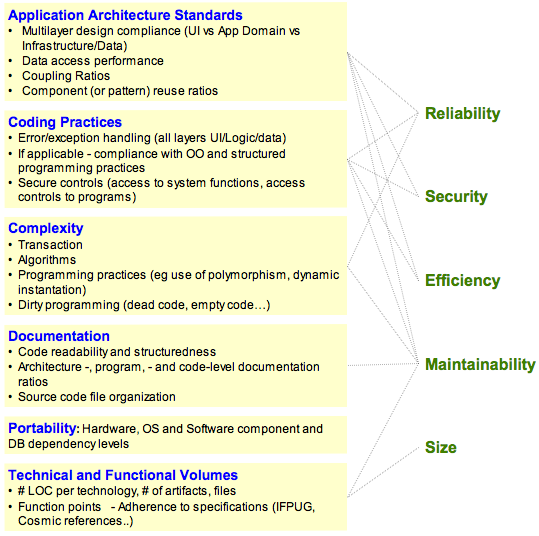
\includegraphics[width=0.9\textwidth]{SoftwareQuality}
        \caption{Software de Calidad}
        \label{fig:softwarequality}
    \end{center}
\end{figure}

\par Un software hecho para ejecutarse una sola vez no requiere el mismo nivel de calidad mientras que un software para ser explotado durante un largo necesita ser fiable, seguro, mantenible y flexible para disminuir los costes.

\begin{itemize}
	\item \emph{Mantenibilidad}: El software debe ser diseñado de tal manera, que permita ajustarlo a los cambios en los requerimientos. Esta característica es crucial, debido al inevitable cambio del contexto en el que se desempeña un software.
	\item \emph{Fiabilidad}: Incluye varias características además de la fiabilidad, como la aplicación de estándares, complejidad, tratamiento de errores.
	\item \emph{Eficiencia}: Tiene que ver con el uso eficiente de los recursos que necesita un sistema para su funcionamiento.
	\item \emph{Seguridad}: La evaluación de la seguridad requiere un control sobre la arquitectura, el diseño y las buenas prácticas.
\end{itemize}

% section software-calidad (end)

\section{Proceso iterativo}
\label{sec:proc-iterativo}

\par ¿ Que es el proceso iterativo ?

\begin{quote}
    \emph{La primera versión debe contener todos los requerimientos del usuario y lo que se va a hacer en las siguientes versiones es ir mejorando aspectos como la funcionalidad o el tiempo de respuesta.}\footnote{Procesos Iterativos e Incrementales - \url{http://esalas334.blogspot.es/1193761920/}}
\end{quote}

\par Se centra más en la inmediatez de la primera versión y en las mejoras posteriores que se van creando enfocadas a la solución final. En el proceso también juega una parte fundamental la comunicación con el cliente a través de la visualización de los resultados por iteraciones. De esta forma se consigue una buena coordinación entre el cliente y el equipo de desarrollo para la consecución de los objetivos.

\begin{figure}[H]
    \centering
    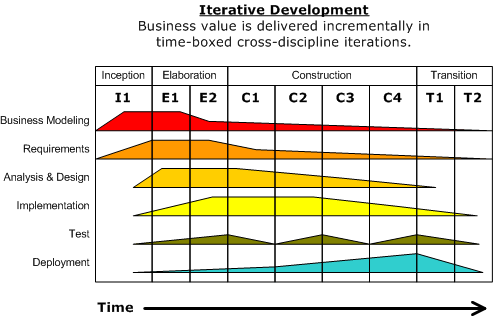
\includegraphics[width=0.9\textwidth]{DevelopmentIterative}
    \caption{Desarrollo Iterativo}
    \label{fig:desarrollo-iterativo}
\end{figure}

\par Se han de tener en cuenta posibles cambios entre iteraciones pero nunca del resultado completo, para que de esta forma se pueda controlar a tiempo la \emph{desviación} que pueda existir en el proceso de la creación de producto.

\begin{quote}
    \emph{Como la idea que representa la palabra iterativo, un proceso de desarrollo de software iterativo es aquel al que se lo piensa, como una serie de tareas agrupadas en pequeñas etapas repetitivas. Estas "pequeñas etapas repetitivas" son las iteraciones.}\footnote{Proceso de Desarrollo Iterativo - Fernando Soriano - \url{http://fernandosoriano.com.ar/?p=13}}
\end{quote}

\par La base el proceso de desarrollo Iterativo provee un conjunto de pasos para el desarrollo de la solución que se repiten iteración tras iteración para la creación de mejoras tangibles y/o evaluables. 

\begin{figure}[H]
    \centering
    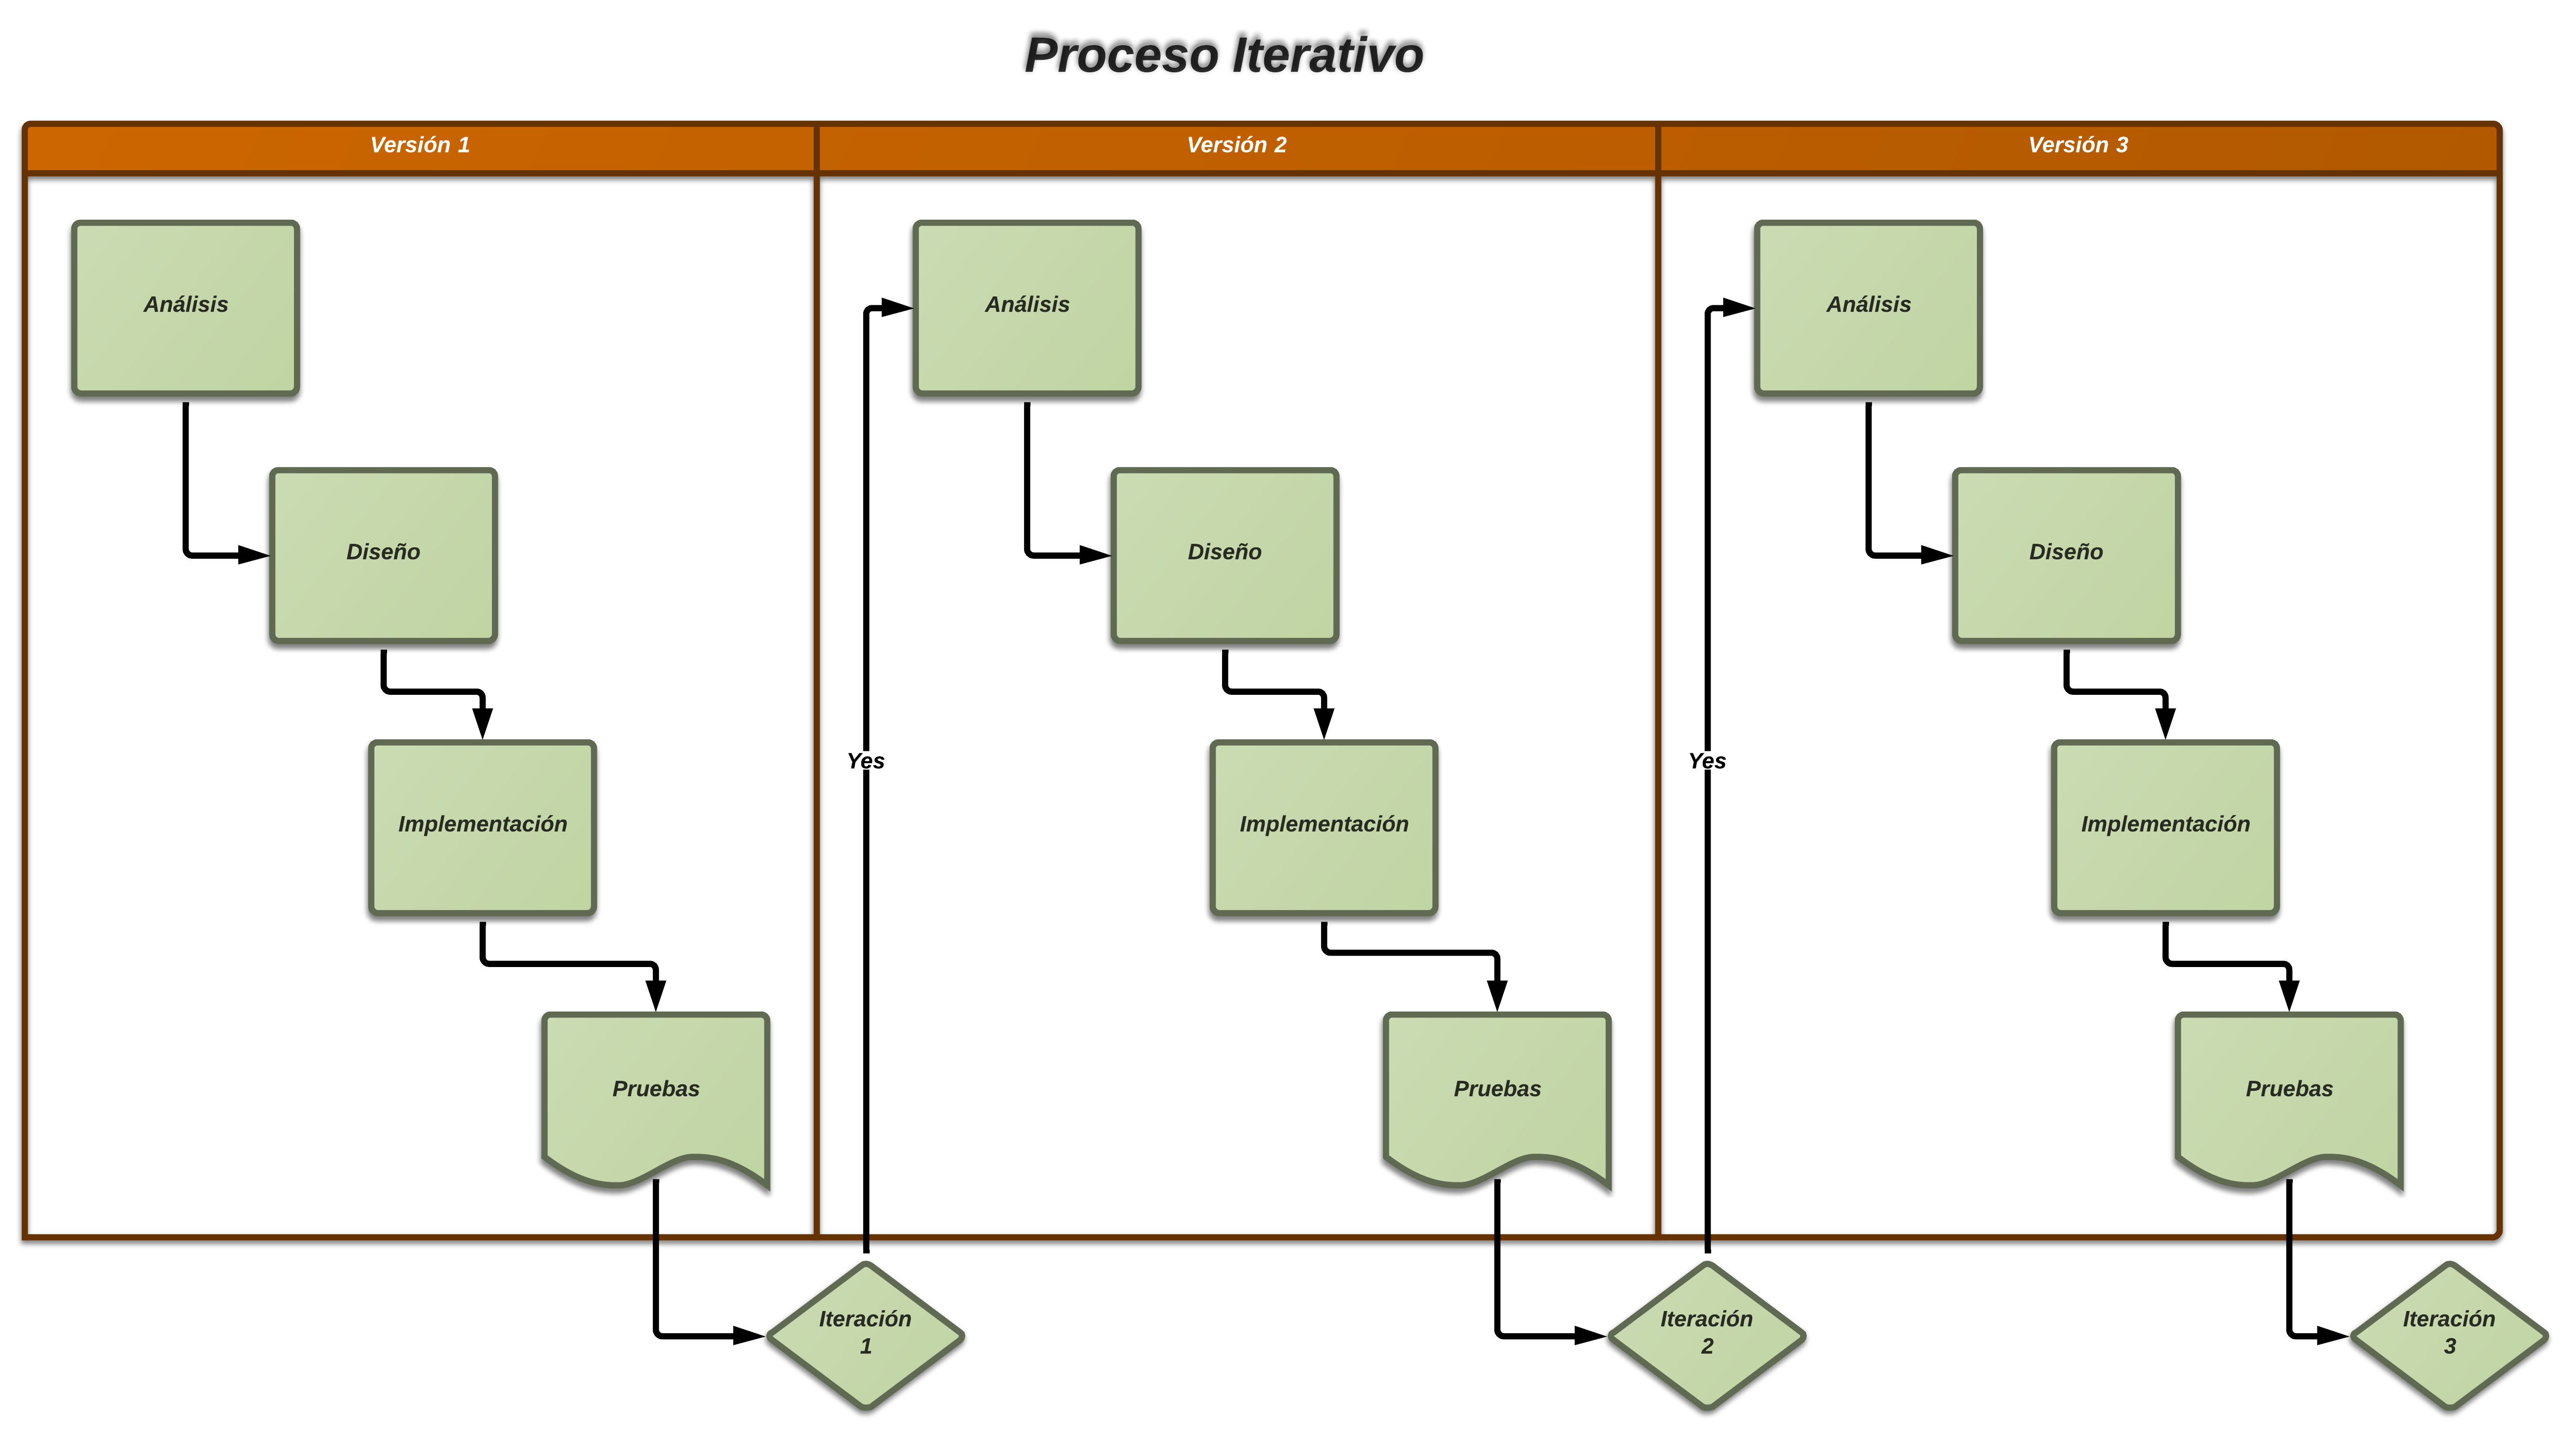
\includegraphics[width=0.9\textwidth]{ProcesoIterativo}
    \caption{Proceso Iterativo}
    \label{fig:ProcesoIterativo}
\end{figure}

\par En cada iteración se construye una pieza funcional del producto final, completa, testeada, documentada e integrada en la solución final. La visión completa de este proceso muestra una línea de iteraciones separadas funcionalmente unas de otras que en conjunto, forman la solución final. Iteraciones independientes unas de otras a través de un desarrollo lineal agrupando pequeños ciclos de desarrollo.

\begin{itemize}
	\item \emph{Duración fija}, quiere decir que una vez establecidos los tiempos o planificación de la iteración, la iteración termina en la fecha exacta establecida. Si el equipo no pudo cumplir lo planificado, el desarrollo pendiente pasa a otra iteración.
	\item Estimación de tiempos cortos, las \emph{"buenas prácticas"} hablan de que una iteración debiera durar entre 2 y 6 semanas.
	\item Es como un ciclo de desarrollo completo, ya que en una iteración se realizan actividades de análisis, diseño, implementación, pruebas, etc.
\end{itemize}

% section proc-iterativo (end)

\section{Proceso incremental}
\label{sec:proc-incremental}

\par El Proceso Incremental fue propuesto por \emph{Harlan D. Mills} en 1980.

\par Sugirió el enfoque incremental de desarrollo como una forma de reducir la repetición del trabajo en el proceso de desarrollo y dar oportunidad de retrasar la toma de decisiones en los requisitos hasta adquirir experiencia con el sistema.

\par El modelo incremental combina elementos del modelo lineal secuencial (aplicados repetidamente) con la filosofía interactiva de construcción de prototipos. El modelo incremental aplica secuencias lineales de forma escalonada mientras progresa el tiempo en el calendario.

\par Cada secuencia lineal produce un \emph{"incremento"} en el desarrollo de la solución. Por ejemplo, en relación a la forja SidelabCode Stack; en la primera versión estaba accesible el módulo de Jenkins, en el siguiente incremento la configuración de Jenkins se ligaba automáticamente a la configuración del los usuarios por proyecto, el siguiente incremento se publicaban las instrucciones para gestionar Jenkins a partir de una cuenta y facilitar la configuración para los distintos entornos.

\begin{figure}[H]
    \centering
    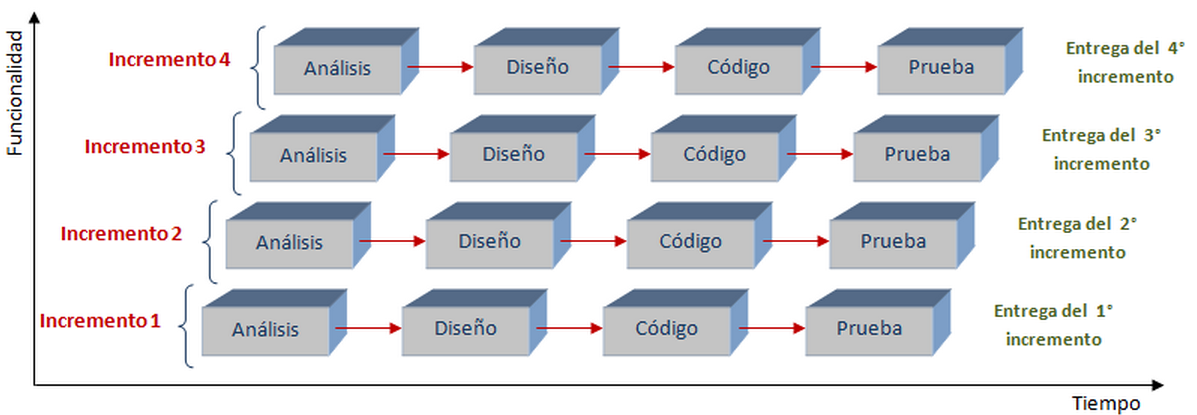
\includegraphics[width=0.9\textwidth]{modelo_incremental}
    \caption{Modelo Incremental}
    \label{fig:modelo-incremental}
\end{figure}

\par Al iniciar el desarrollo, los clientes o los usuarios, identifican a grandes rasgos las funcionalidades que proporcionará el sistema. Se define un bosquejo de requisitos funcionales y será el cliente quien se encarga de priorizar que funcionalidades son más importantes. Con las prioridades definidas, se puede confeccionar el plan de incrementos, en donde cada incremento se compone de un subconjunto de funcionalidades a desarrollar.

% section proc-incremental (end)

\section{Iterativo e Incremental}
\label{sec:iterativo-incremental}

\par Desarrollo iterativo e incremental. La conjunción de estos dos tipos de desarrollo aúnan las mejores cualidades de ambos para gestión de un equipo de trabajo en la construcción de una solución.

\par El proceso iterativo e incremental se basa en incrementos por cada una de las iteraciones en el proceso de desarrollo. La idea básica de este proceso es desarrollar una solución a través de las iteraciones de ciclos a partir de los incrementos en la funcionalidad para que los desarrolladores mejoren su productividad en torno al proyecto a partir de pequeños hitos que completan versiones usables de la solución desde la primera implementación.

\begin{figure}[H]
    \centering
    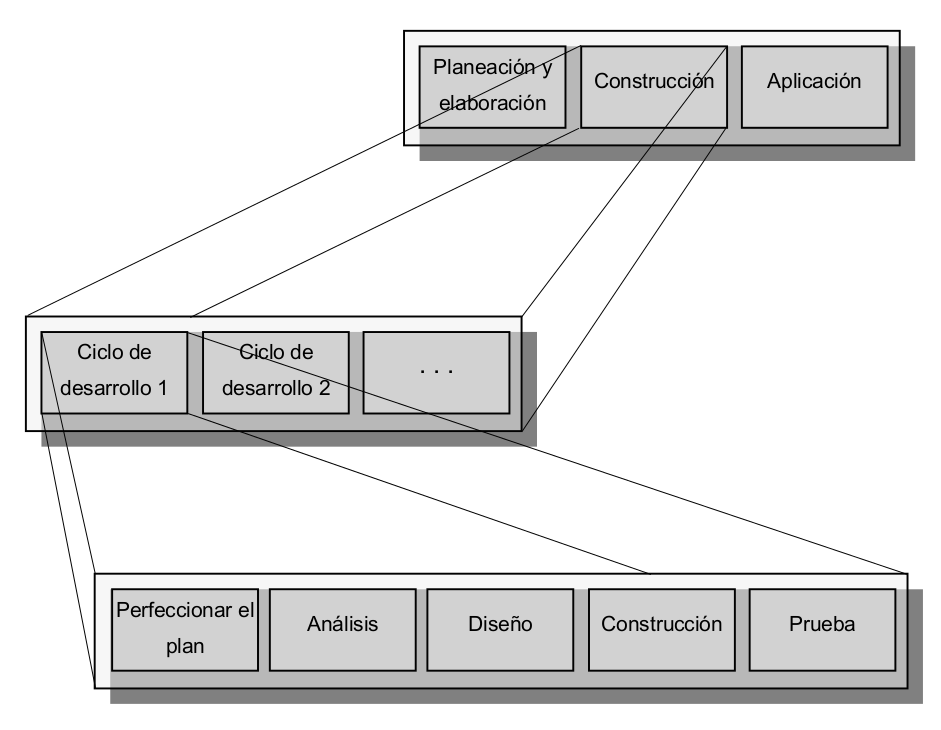
\includegraphics[width=0.9\textwidth]{iterativo-incremental-larman}
    \caption{Proceso iterativo e Incremental por Larman}
    \label{fig:iterativo-incremental-larman}
\end{figure}

\par La evolución de la solución se basa en las iteraciones pasadas añadiendo los nuevos requisitos/objetivos (pueden ser mejoras o nuevas funcionalidades). Se basa en incrementar el valor del trabajo hecho para tener un control del proceso más exhaustivo priorizando los objetivos. Por cada iteración existen modificaciones en el diseño y en las funcionalidades.

\par La comunicación y la implicación en el desarrollo del proyecto con el usuario/cliente desde el inicio del proyecto es crucial ya que el proceso parte desde una solución inicial para incluir versiones usables con el usuario/cliente. De esta forma todas las partes aportan sus distintos puntos de vista de una manera continua implicándose en el proceso y midiendo el crecimiento de la solución paso a paso, incremento a incremento.

\par Este proceso de desarrollo cercano a las \emph{Metodologías Ágiles}, como ellas tiene el mismo fin, la implicación, desarrollo, fiabilidad, confianza, aprendizaje, versatilidad, responsabilidad, comunicación con la solución desarrollada y el usuario/cliente durante el proceso.

\par Una de las claves en este proceso es la retroalimentación y el aprendizaje del grupo de trabajo a partir de las iteraciones. De esta forma el trabajo hecho repercute en las iteraciones futuras aportando nuevos conocimientos sobre el proceso y el desarrollo. Creando mejores iteraciones y evoluciones de la solución, \emph{profesionalizando el trabajo}.

\par Las Iteraciones han de ser de una duración corta de \emph{2 a 6 semanas} para que la comunicación a todos los niveles del proyecto siga siendo fluida y para que si en algún caso se haya de desechar una Iteración no se pierda mucho trabajo desarrollado en ella. Esto no ocurre muy a menudo pero se contempla por diferentes causas:

\begin{itemize}
	\item Abandono del proyecto.
	\item Cambio de Cliente/Usuario.
	\item Falta de recursos.
\end{itemize}

\par Las Iteraciones \emph{"cortas"} otorgan al modelo un alto nivel de versatilidad a la hora de evolucionar y evaluar el recorrido del trabajo hecho en el proyecto, para así poder predecir la organización de las futuras iteraciones.

\subsection{Fases del proceso}
\label{sub:fases-proceso}

\par El proceso de desarrollo Iterativo e Incremental está basado en tres fases:

\begin{itemize}
	\item Iniciación.
	\item Iteración.
	\item Lista del Control del Proyecto.
\end{itemize}

\par El objetivo de la \emph{Iniciación} es la implementación inicial para crear un producto con el cual el usuario/cliente pueda interactuar y tener las primeras impresiones. El equipo de desarrollo y el usuario/cliente toman como punto base esta fase de \emph{Iniciación}.

\par Esta primera implementación ha de servir de guía para la evolución del desarrollo en cada una de las iteraciones, la base.

\par La \emph{Lista de Control del Proyecto} es el lugar donde se definen las tareas que han de cumplimentarse durante el proceso de desarrollo. Todos los aspectos relacionados con la implementación de la solución se encuentran definidos en la lista, funcionalidades, diseño, errores, mejoras. La Lista de Control está en constante evolución, no es un muro estático, ya que se van adjuntando las funcionalidades y/o mejoras y posibles nuevas funcionalidades. De esta forma se evalúan las prioridades en la fase de análisis por cada iteración y se decide que tareas han de implementarse y cuales son desechadas para la siguiente iteración.

\par La \emph{Iteración} es un conjunto modular de acciones a llevar a cabo para cumplir con las tareas que se definen para evolucionar la solución por incrementos. Debe estar sujeta a cambios en el diseño, nuevas tareas añadidas a la lista de control y sobretodo, ser simple.

% subsection fases-proceso (end)

\subsection{Desarrollo Iteración}
\label{sub:desarrollo-iteracion}

\par El desarrollo del proyecto viene medido por las Iteraciones que se conectan una a otra secuencialmente.

\par La iteración comienza a partir del análisis basado en la retroalimentación de los usuarios y los servicios de análisis disponibles. Los elementos a tener en cuenta en el análisis son:

\begin{itemize}
	\item Estructura.
	\item Modularidad.
	\item Ergonomía.
	\item Eficiencia.
	\item Objetivos logrados.
\end{itemize}

\par Se han tener en cuenta los posibles riesgos que puedan surgir en la Iteración para evaluarlos y eliminarlos en el momento de definir la línea base de la arquitectura. Además el equipo de desarrollo ha de dominar y estar al tanto del lenguaje empleado en los requisitos, el problema que se va a abordar y de esta manera ser capaces de asumir los posibles riesgos o imprevistos que puedan surgir.

\par Los resultados del análisis se reflejan en la Lista de Control del proyecto para añadir, modificar y ordenar por prioridades para la siguiente Iteración.

\begin{figure}[H]
    \centering
    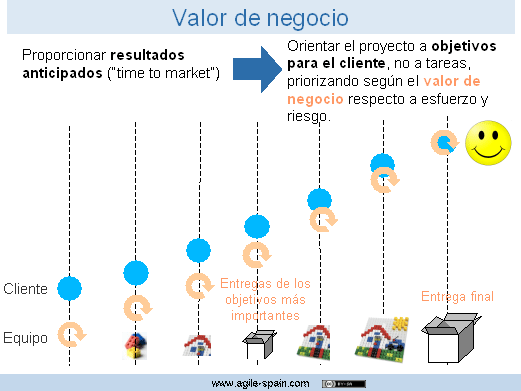
\includegraphics[width=0.9\textwidth]{valor-negocio-iterativo-incremental}
    \caption{Valor de negocio Iterativo e Incremental}
    \label{fig:valor-negocio-iterativo-incremental}
\end{figure}


\par En las Iteraciones posteriores ha de aumentar la capacidad de reducir los riesgos, desarrollar los componentes e ir evolucionando incremento a incremento hacia la versión final para el usuario/cliente.

\par Cada Iteración se reduce a un \emph{miniproyecto} (Se les llama miniproyectos porque no es algo que el usuario haya pedido) que consta del proceso de requisitos, análisis, diseño, implementación y prueba.

\par El proceso de desarrollo en una Iteración se reduce a una serie de guías o pasos a seguir en torno a las modificaciones que surgen a la medida que se avanza en el desarrollo. El proceso Iterativo e Incremental se basa en la flexibilidad por lo tanto las modificaciones de la Iteración han de ser otra herramienta más para lograr los objetivos y como tales:

\begin{itemize}
	\item Cualquier dificultad encontrada en el diseño, desarrollo y prueba de una modificación puede alertar de la necesidad de cambiar el diseño o la implementación. Se han de desarrollar las modificaciones con una estructura modular y aislada (en su medida) para poder trabajar en un problema o solución concreta y que no afecte al resto de la implementación.

	\item Las modificaciones han de ser sencillas de implementar, sino se ha de rediseñar el la solución.

	\item Las modificaciones han de ser más sencillas conforme se van completando iteraciones. Si esto no ocurre existe un problema de diseño y puede incurrir en el exceso de soluciones \emph{ad-hoc}, parches.

	\item Los parches se contemplan como soluciones temporales en distintas iteraciones para que no sea necesario un cambio en el diseño, pero sólo para casos excepcionales. Si los parches proliferan se ha de replantear el diseño.

	\item La implementación existente ha de ser analizada constantemente para certificar que sigue el camino marcado por los objetivos a corto y largo plazo del proyecto. De esta forma se controlan las posibles desviaciones de tiempo y el trabajo hecho por el grupo de trabajo.

	\item Los herramientas de análisis se han de utilizar para validad los análisis y/o funcionalidades de las implementaciones parciales de la solución.

	\item La participación del usuario/cliente en el proceso ha de ser solicitada y analizada para contemplar posibles deficiencias o errores en la implementación actual. De esta forma es como se ha de crear una canal de comunicación para interactuar con el grupo de trabajo.

\end{itemize}

% subsection desarrollo-iteracion (end)


% section iterativo-incremental (end)
\section{Gestión de tareas}
\label{sec:gestion-tareas}

\par Gestión de tareas: ¿qué hay que hacer? ¿quién tiene que hacerlo? -> Sistemas de gestión de tickets
% section gestion-tareas (end)

\section{Código versionado}
\label{sec:codigo-versionado}

\par Código versionado -> repositorios de código

% section codigo-versionado (end)

\section{TDD y CI}
\label{sec:tdd-ci}

\par TDD -> sistemas de CI para asegurar que los tests se pasan regularmente

% section tdd-ci (end)

\section{Desarrollo por canales}
\label{sec:desarrollo-canales}

% section desarrollo-canales (end)

\section{Herramientas}
\label{sec:herramientas}

% section herramientas (end)


%%%%%%%%%%%%%%%%%%%%%%%%%%%%%%%%%%%%%%

\chapter{ALM Tools}
\label{chap:almtools}

* ALM Tools - Forjas de desarrollo
    * Qué es una forja
    * Objetivos
    * Componentes
        * Estudio del arte de forjas
    * Problemática -> administración, costes...
        * Tablas comparativas
    * Algunos ejemplos y sus limitaciones
    * Conclusiones del estudio de forjas

\par ALM Tools significa: \emph{Application Lifecycle Management Tools}. La gesti\'on del ciclo de vida de una aplicaci\'on, el conjunto de herramientas encargadas de gu\'iar al desarrollador a trav\'es de un camino basado en metodolog\'ias para la creaci\'on de un Software hacia su estado del arte.

\par Integrar el proceso de desarrollo de Software a trav\'es de las ALM Tools como veh\'iculo, es decir no existe en si mismo una herramienta ALM, sino que la herramienta ALM gobierna a las herramientas incluidas en el proceso de desarrollo.

\section{Historia}
\label{sec:historia}

\par En todas las empresas o comunidades que desarrollan Software siempre se aplica un proceso de desarrollo a la creación del producto. Cada una utiliza distintas herramientas para la gesti\'on de los proyectos de Software, gestor de correo, gestor de incidencias, repositorio de c\'odigo, integraci\'on continua. Pero en la mayor\'ia de los casos de una forma dispar y sin seguir ninguna convención.

\par A veces el no conocimiento de otras herramientas o la no inclusión de nuevas puede hacer que el desarrollo del proyecto no mejore, partiendo de la base de que el desarrollo puede ser óptimo para las herramientas utilizadas, carece de perspectivas de mejora a corto plazo.

\par Si se opta por la integración de una nueva herramienta en el proceso de desarrollo el coste de integración se habría de evaluar ya que se debería dedicar un esfuerzo a la integración ad-hoc de la nueva herramienta para el uso en este mismo entorno con el coste que conlleva, evaluación, test, integración, interoperabilidad, es decir un nuevo proyecto dentro del mismo proyecto.

\par Después de esta integración en el proceso de desarrollo en la empresa habría que hacer un esfuerzo para salvaguardar la información a través de las distintas herramientas por separado.

\par El proceso de unificación y reutilización de herramientas a los desarrolladores nos puede parecer familiar si lo comparamos con el uso de los Frameworks a principios de los años 2000. Muchas empresas o comunidades empezaron a adecuar e implementar sus desarrollos en base a un Framework creado por ellos mismos. Estos Frameworks se adecuan a sus requerimientos pero su uso era interno en la empresa y por lo tanto lejano a los estándares. Uno de los más famosos es sin duda el caso de Spring, proyecto de más de 10 años de edad que goza de buena salud y aceptación, incluso equivoca a algunos entre Java y Spring. En este pequeño paralelismo podemos encontrar el estado de las forjas de desarrollo ALM Tools, cuando el proyecto requiere de herramientas para facilitar su ciclo de vida y se van ensamblando una tras otra, que perfectamente las podemos llamar librerías, en una integración \textbf{ad-hoc} y siguiendo unos pasos repetitivos en cada nuevo proyecto, en los que humanamente todos nos podemos equivocar debido a que depende de cada uno seguir cada uno de los pasos. Estas herramientas tienden a convertirse en pequeños estándares dentro de cada grupo de desarrolladores y a repetirse en futuros proyectos, pero debido a los desarrollos \textbf{ad-hoc} carecen de escalabilidad e integración con nuevas soluciones de una forma ágil, es un escollo actualizar y por otro lado replicar un estándar para la implantación de la forja, no se tiende a dejar puertas abiertas para que más adelante el herramienta mejore. Se podría definir como uno de los casos de inanición en el desarrollo de Software o muerte por éxito.

\par En este punto es donde entra la famosa interoperabilidad entre las herramientas, la necesidad de interoperabilidad entre la herramientas a través de una comunicación estándar. Aquí encontramos el punto clave de las ALM Tools, la \textbf{integración de herramientas} dentro de un proceso de desarrollo.

\par En post de evitar la falta de replicación, además de la importancia de la interoperabilidad se ha de tener en cuenta la replicación del contenido o la gestión de la instalación de un ALM. Siempre se ha de pensar mirando hacia adelante, no es necesario implementar las mejoras pero sí, dejar un hueco para que casen bien. Un ejemplo que puede ilustrar esta frase es la programación basada en Interfaces mediante Java, ya que las Intefaces ofrecen soluciones para implementar a medida y si se actualiza la Interfaz (en este caso es el esqueleto de la clase) para añadir una nueva funcionalidad con un método, los métodos anteriores mantienen su comportamiento dentro de cada clase que la implementa y adquieren la posibilidad de aumentar la funcionalidad implementando la nueva solución, adecuada a su entorno pero nueva, de esta forma la interoperabilidad entre las clases que utilicen esta Interfaz también se mantiene.

% subsection historia (end)


\section{Qué es una forja}
\label{sec:que-es}

% section que-es (end)

\section{Objetivos}
\label{sec:objetivos}

% section objetivos (end)

\section{Componentes}
\label{sec:componentes}

\par Este conjunto de herramientas se puede dividir en varios grupos:

\begin{itemize}
	\item Gesti\'on de Requisitos.
	\item Arquitectura.
	\item Desarrollo.
	\item Test.
	\item Issue tracking system.
	\item Continuous Integration.
	\item Release Management.
\end{itemize}

\par Hoy en d\'ia las forjas ALM abundan, adem\'as de gozar de una gran popularidad entre los proyectos de Software, como podemos ver en los casos de SourceForge, Googlecode y Github (más adelante discutiremos cada proyecto). En este caso ALM Tools as a Service, debido al servicio que ofrecen, pero sólo las que son FLOSS permiten replicar ese mismo entorno en tu propia máquina, un dato muy importante a tener en cuenta, porque siempre se ha de mirar hacia adelante.

% subsection componentes (end)

\section{Estado del arte de forjas}
\label{sec:estado-del-arte}

\begin{itemize}
	\item ClinkerHQ \url{http://clinkerhq.com/} - Privado.
	\item Github - \url{http://github.com/} - Privado.
	\item SourceForge con Allura - \url{http://sourceforge.net/projects/allura/} - Software Libre pero incompleta (integrated Wiki, Tracker, SCM (svn, git and hg), Discussion, and Blog tools).
	\item Cloudbees DEV@Cloud \url{http://www.cloudbees.com/dev.cb} - Privado.
	\item CollabNet con CloudForge \url{http://www.cloudforge.com/} - Privado.
	\item Plan.io - \url{http://plan.io/en/} - Privado.
	\item Bitnami - \url{http://bitnami.com/} - Privado
	\item GForge
	\item Collab.net
	\item Google Code
	\item Bitbucket - https://bitbucket.org/mswlmanage2013/mswl-bitbucket-alm-tools/wiki/Home
\end{itemize}

% subsection estado-del-arte (end)

\subsection{Problemas en algunas forjas}
\label{sub:problemas}

% subsection problemas (end)

\subsection{Tablas comparativas}
\label{sub:comparativa}

% subsection comparativa (end)

\section{Conclusiones del estudio de forjas}
\label{sec:conclusiones}

% subsection conclusiones (end)


%%%%%%%%%%%%%%%%%%%%%%%%%%%%%%%%%%%%%%

%%%%%%%%%%%%%%%%%%%%%%%%%%%%%%%%%%%%%%%%%%%%%%%%%%%%%%%%%%%%%%%%%%%%%%%%%%%%%%%%%%%%%%%%%%%%%%%%%%%%%%%%%%%
%   \copyright 2013 Ricardo García Fernández - ricardogarfe [at] gmail [dot] com.
%
%    This work is licensed under a Creative Commons 3.0 Unported License.
%    To view a copy of this license visit:
% 
%    http://creativecommons.org/licenses/by/3.0/legalcode
%%%%%%%%%%%%%%%%%%%%%%%%%%%%%%%%%%%%%%%%%%%%%%%%%%%%%%%%%%%%%%%%%%%%%%%%%%%%%%%%%%%%%%%%%%%%%%%%%%%%%%%%%%

%%%%%%%%%%%%%%%%%%%%%%%%%%%%%%%%%%%%%%%%%%%%%%%%%%%%%%%%%%%%%%%%%%%%%%%%%%%%%%%%%%%%%%%%%%%%%%%%%%%%%%%%%%
% SCStack
%%%%%%%%%%%%%%%%%%%%%%%%%%%%%%%%%%%%%%%%%%%%%%%%%%%%%%%%%%%%%%%%%%%%%%%%%%%%%%%%%%%%%%%%%%%%%%%%%%%%%%%%%%

\chapter{SCStack}
\label{chap:scstack}

\par SCStack es el conjunto de herramientas que componen la Forja de desarrollo. La palabra \emph{stack} en Inglés significa \emph{pila}, con respecto a la forja se trata del conjunto de herramientas apiladas y conectadas que dan forma a la Forja.

\begin{figure}[H]
    \centering
    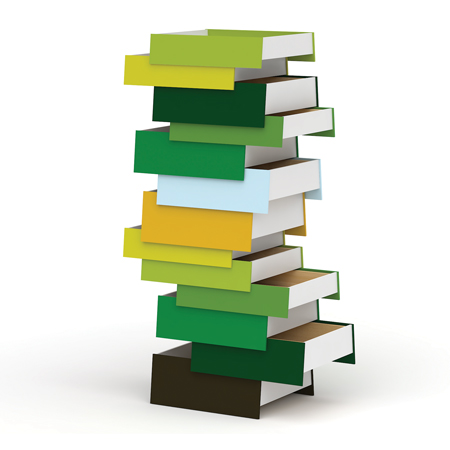
\includegraphics[width=0.7\textwidth]{stackstorage}
    \caption{Ejemplo de pila a partir de cajones}
    \label{fig:stackstorage}
\end{figure}

\section{Arquitectura}
\label{sec:arquitectura}

\par La arquitectura del Sistema de Gestión de la Forja se ve reflejada en el siguiente esquema:

\begin{figure}[H]
    \centering
    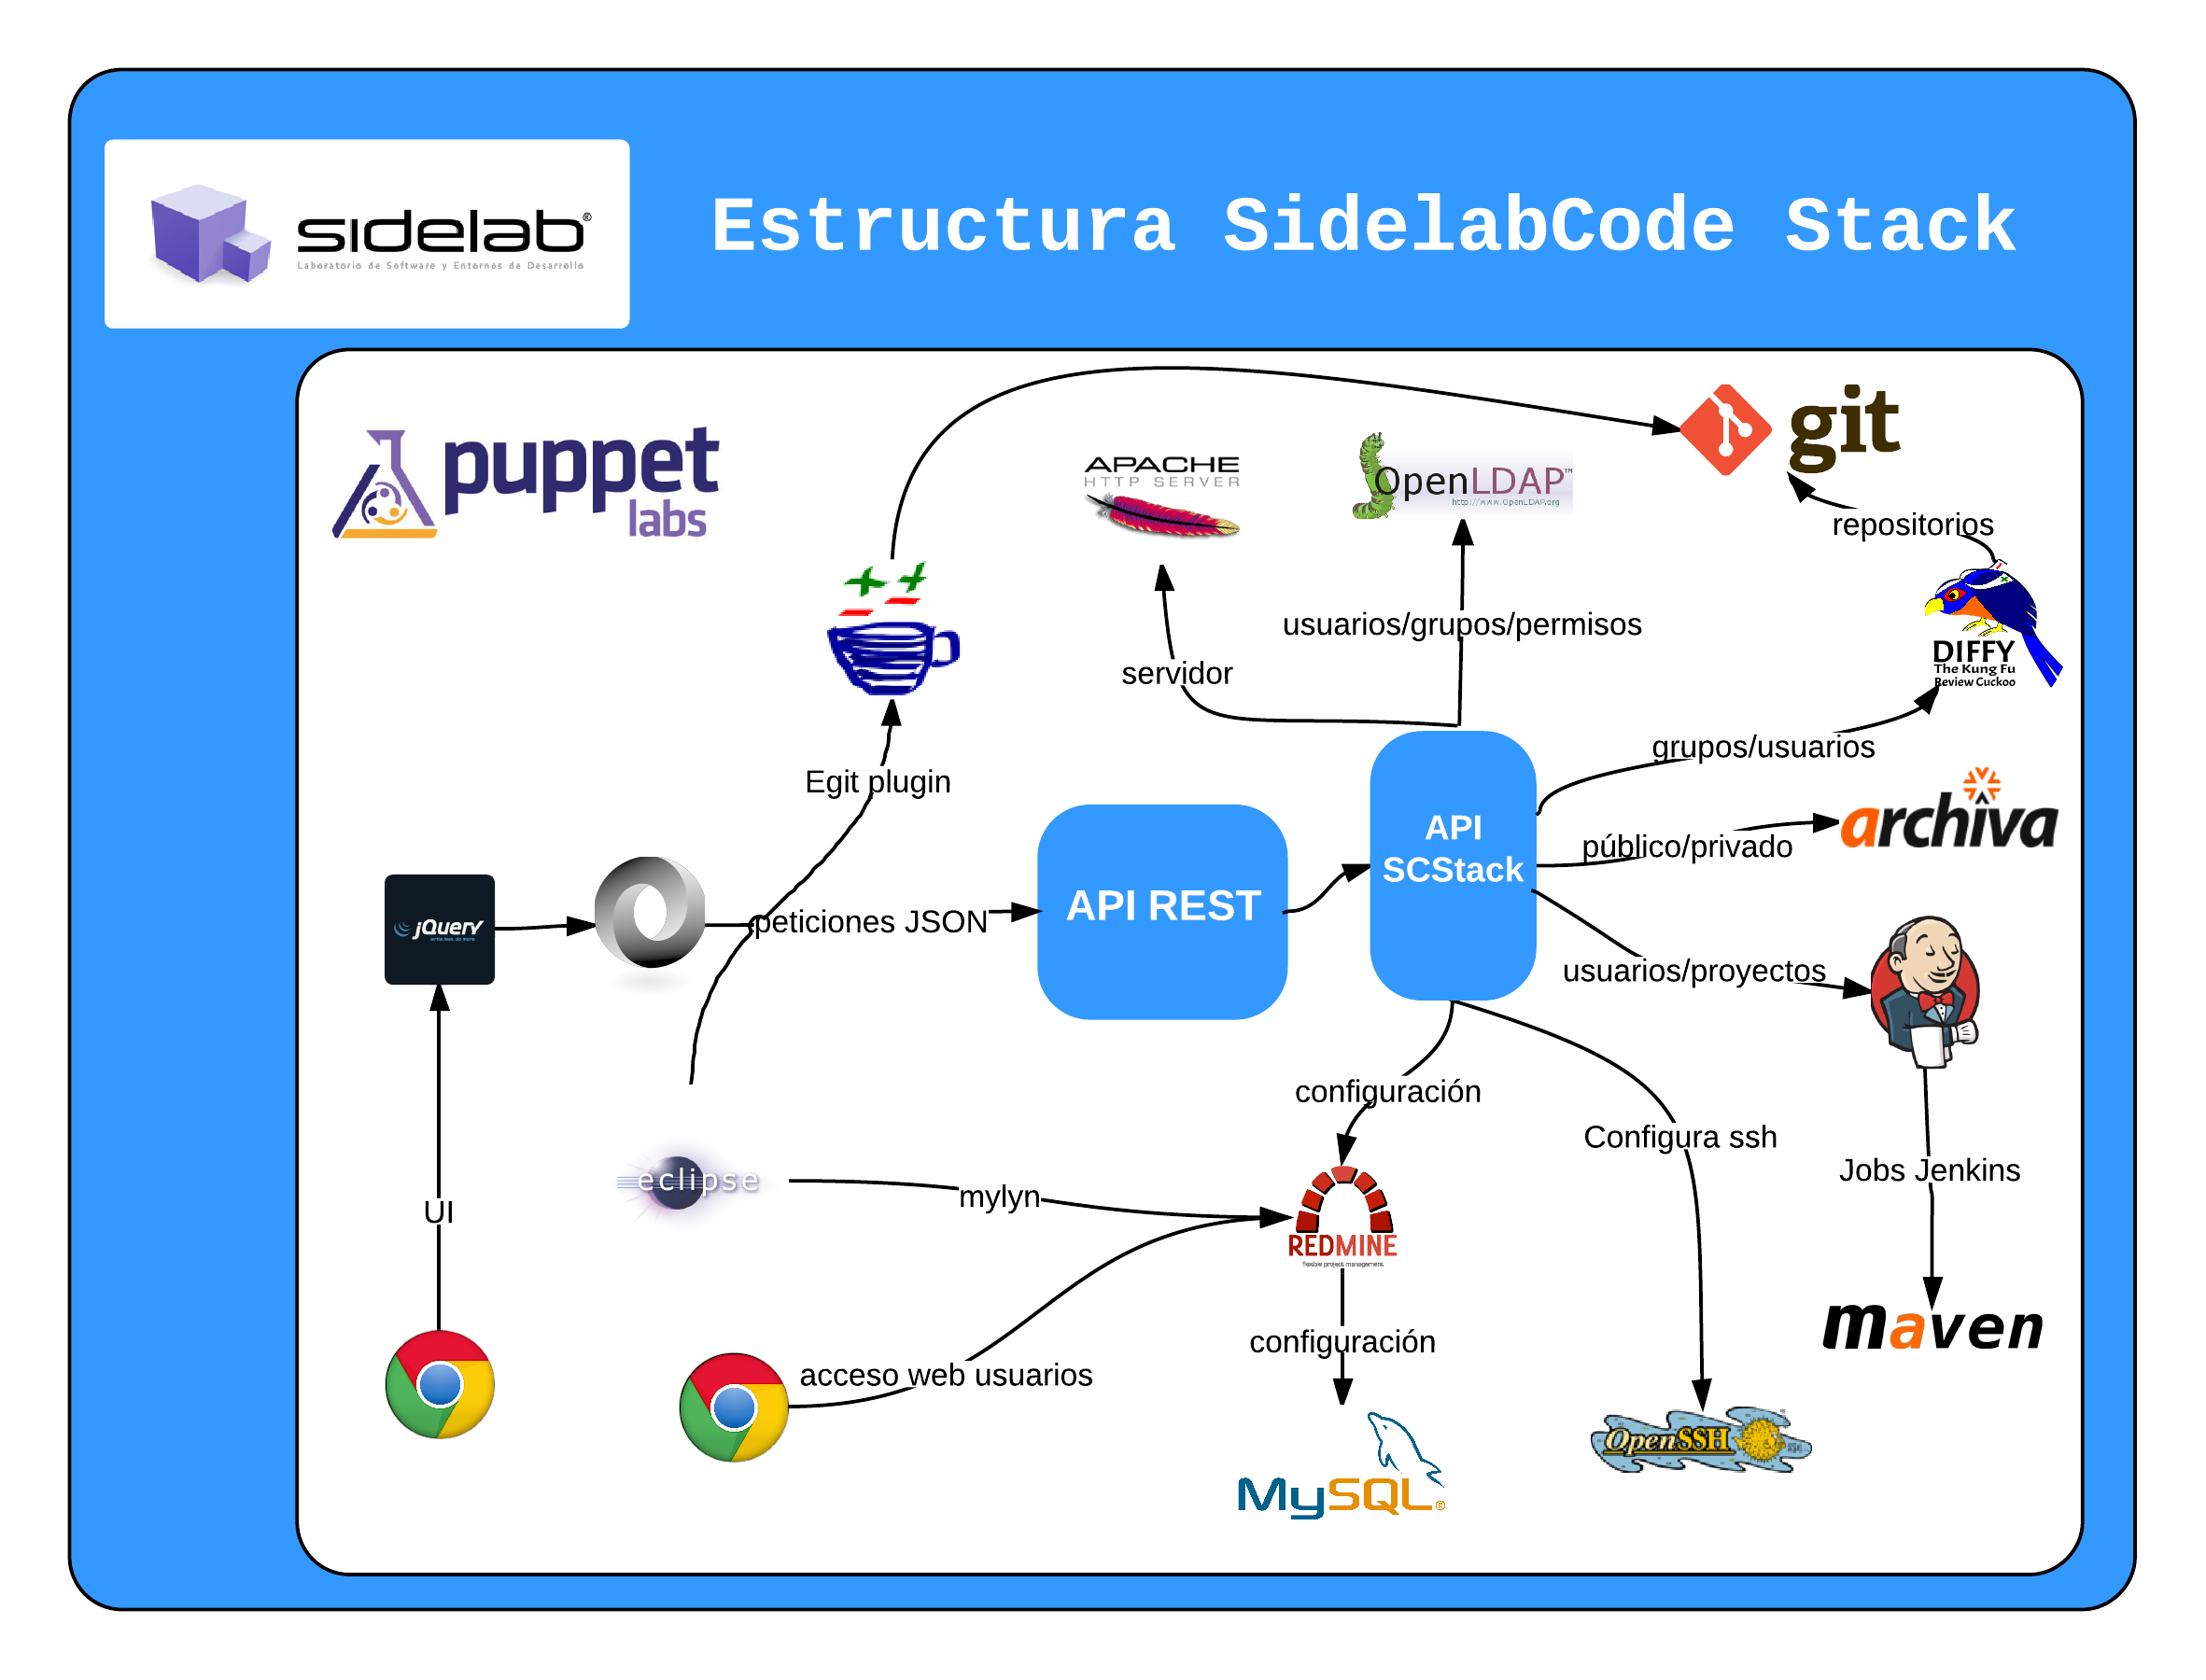
\includegraphics[width=\textwidth]{scstack-diagram}
    \caption{Diagrama de arquitectura SCStack}
    \label{fig:scstack-diagram}
\end{figure}

\par El proyecto consta de tres componentes conectados entre sí para la comunicación del usuario con las herramientas para la gestión de los proyectos: La Consola de Administración, el servidor de servicios web REST y el API.

%%%%%%%%%%%%%%%%%%%%%%%%%%%%%%%%%%%%%%%%%%%%%%%%%%%%%%%%%%%%%%%%%%%%%%%%%%%%%%%%%%%%%%%%%%%%%%%%%%%%%%%%%%
% Consola de Administración
%%%%%%%%%%%%%%%%%%%%%%%%%%%%%%%%%%%%%%%%%%%%%%%%%%%%%%%%%%%%%%%%%%%%%%%%%%%%%%%%%%%%%%%%%%%%%%%%%%%%%%%%%%

\subsection{Consola de Administración}
\label{sub:consola-admin}

\par \textbf{Consola de Administración}: Se trata de la capa de la vista encargada de interactuar con el usuario. A través de la interfaz que se ejecuta sobre un navegador web, el usuario administrador gestiona los usuarios y los proyectos de la Forja: crear, editar, modificar, eliminar y buscar), el típico sistema CRUD-F\footnote{\url{http://en.wikipedia.org/wiki/Create,\_read,\_update\_and\_delete}} (\emph{CRUD: Create, Read, Update and Delete also Find}). Está diseñada con el framework Javascript \emph{jQuery} por lo que no requiere ninguna librería externa para su uso, únicamente el navegador del cliente. Las operaciones que se realizan en la capa UI se trasladan al servidor REST a través de peticiones \emph{http} asíncronas mediante las interfaces REST definidas.

% subsection consola-admin (end)

%%%%%%%%%%%%%%%%%%%%%%%%%%%%%%%%%%%%%%%%%%%%%%%%%%%%%%%%%%%%%%%%%%%%%%%%%%%%%%%%%%%%%%%%%%%%%%%%%%%%%%%%%%
% Servicio web REST
%%%%%%%%%%%%%%%%%%%%%%%%%%%%%%%%%%%%%%%%%%%%%%%%%%%%%%%%%%%%%%%%%%%%%%%%%%%%%%%%%%%%%%%%%%%%%%%%%%%%%%%%%%

\subsection{Servicio web REST}
\label{sub:rest-ws}

\par \emph{REST}: Representational State Transfer se trata de una arquitectura acuñada por \emph{Roy Fielding}\footnote{\url{http://roy.gbiv.com/}}, uno de los autores de la especificación del protocolo \emph{HTTP}. Esta arquitectura de comunicación se basa en cuatro principios:

\begin{itemize}
	\item Un protocolo cliente/servidor \emph{sin estado}: cada mensaje HTTP contiene toda la información necesaria para comprender la petición. Como resultado, ni el cliente ni el servidor necesitan recordar ningún estado de las comunicaciones entre mensajes. Sin embargo, en la práctica, muchas aplicaciones basadas en HTTP utilizan cookies y otros mecanismos para mantener el estado de la sesión.

	\item Un \emph{conjunto de operaciones} bien definidas que se aplican a todos los recursos de información: HTTP en sí define un conjunto pequeño de operaciones, las más importantes son \textbf{POST}, \textbf{GET}, \textbf{PUT} y \textbf{DELETE}.

	\item Una sintaxis \emph{universal} para identificar los recursos. En un sistema REST, cada recurso es direccionable únicamente a través de su URI.

	\item El uso de \emph{hipermedios}: tanto para la información de la aplicación como para las transiciones de estado de la aplicación. Como resultado de esto, es posible navegar de un recurso REST a muchos otros, simplemente siguiendo enlaces sin requerir el uso de registros u otra infraestructura adicional.
\end{itemize}

\par El uso de los servicios REST para la comunicación mediante el protocolo http con la Consola de Administración agiliza la adaptación de la funcionalidades al cliente, el tráfico y las posibles adaptaciones de nuevos clientes para el acceso a través de cualquier plataforma.

\begin{figure}[H]
    \centering
    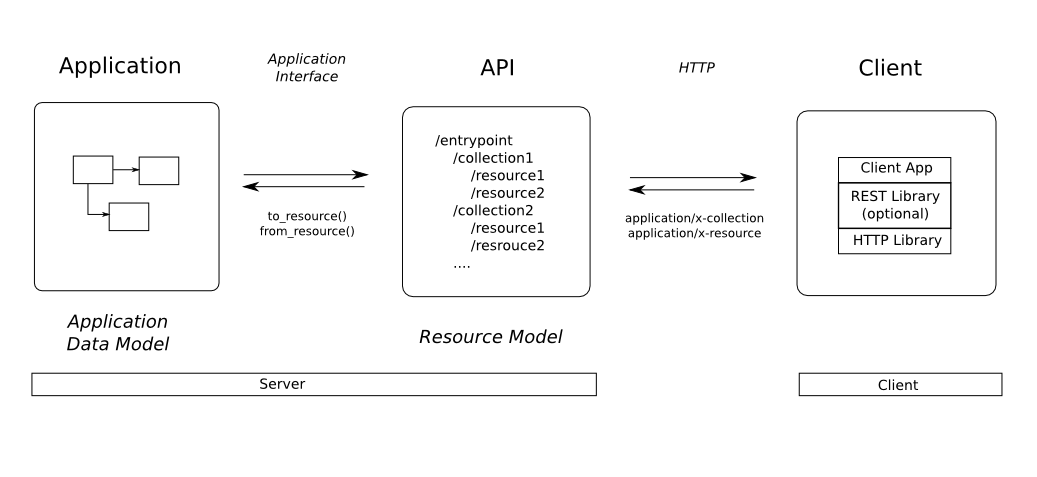
\includegraphics[width=1\textwidth]{rest-scope}
    \caption{Diseño de un API RESTful}
    \label{fig:rest-scope}
\end{figure}

\par \textbf{Servicio web REST}: Es el componente encargado de gestionar las peticiones http a los servicios REST de la Consola de Administración y el API de SidelabCode. Define e implementa la lógica a seguir para la construcción de un proyecto a través de la UI mediante las llamadas ordenadas al API de cada una de las herramientas involucradas en el servicio como componentes de la forja.

\par Los servicios REST ofrecen tres interfaces distintas accesibles a través de http: XML, JSON y HTML para la comunicación la API. Además, hay que desatacar que el servicio web es servido a través del framework \emph{Restlet} a través de Internet de forma continua y remota a cualquier usuario o proceso cliente.

\par Se encarga de la seguridad y validación para las operaciones permitidas o denegadas del usuario de la UI, proporcionando, según su rol, determinados servicios a través de la Consola de Administración, buscar proyectos, crear usuarios, editar proyectos, crear proyectos, etc.

% subsection rest-ws (end)

%%%%%%%%%%%%%%%%%%%%%%%%%%%%%%%%%%%%%%%%%%%%%%%%%%%%%%%%%%%%%%%%%%%%%%%%%%%%%%%%%%%%%%%%%%%%%%%%%%%%%%%%%%
% API
%%%%%%%%%%%%%%%%%%%%%%%%%%%%%%%%%%%%%%%%%%%%%%%%%%%%%%%%%%%%%%%%%%%%%%%%%%%%%%%%%%%%%%%%%%%%%%%%%%%%%%%%%%

\subsection{API}
\label{sub:api}

\par \textbf{API}: La API es el núcleo funcional de SCStack, coordina y realiza las tareas para cada componente de la forja con respecto a los usuarios y proyectos involucrados. Traslada las órdenes ejecutadas en la capa UI a las distintas herramientas para configurar su funcionamiento. Está conectada a todos los servicios que ofrece pivotando a través del directorio LDAP: Control de Versiones, Directorios, Integración Continua, ITS, Revisiones, Gestión de Dependencias, Seguridad y Autenticación que analizaremos extensamente más adelante componente a componente.

% subsection api (end)

% section arquitectura (end)

%%%%%%%%%%%%%%%%%%%%%%%%%%%%%%%%%%%%%%%%%%%%%%%%%%%%%%%%%%%%%%%%%%%%%%%%%%%%%%%%%%%%%%%%%%%%%%%%%%%%%%%%%%
% Aprovisionamiento (Puppet)
%%%%%%%%%%%%%%%%%%%%%%%%%%%%%%%%%%%%%%%%%%%%%%%%%%%%%%%%%%%%%%%%%%%%%%%%%%%%%%%%%%%%%%%%%%%%%%%%%%%%%%%%%%

\section{Aprovisionamiento (Puppet)}
\label{sec:puppet}

\par \emph{Aprovisionamiento}: 'Accción o efecto de aprovisionar', \emph{aprovisionar}: abastecer\footnote{Definición del diccionario de la RAE - \url{http://buscon.rae.es/drae/?type=3&val=aprovisionar&val_aux=&origen=REDRAE}}. Aplicado a la Ingeniería del Software el Aprovisionamiento nos provee de los componentes necesarias para construir una solución.

\par El aprovisionamiento trata de la automatización de tareas para construir el entorno deseado, en este caso la instalación de SidelabCode Stack. La evolución en el modelo de instalación para facilitar la ejecución de módulos, configuración y comunicación entre los distintos componentes.

\par La herramienta empleada para el aprovisionamiento es \textbf{Puppet} de la compañía \emph{PuppetLabs}\footnote{\url{https://puppetlabs.com/}}.

\begin{figure}[H]
    \centering
    
\includegraphics[width=0.3\textwidth]{puppet-labs-logo}
    \caption{Puppet Labs Logo}
    \label{fig:puppet-labs}
\end{figure}

\par \emph{Puppet}: es una herramienta \emph{Software Libre}\footnote{\url{https://puppetlabs.com/puppet/puppet-open-source/}} de aprovisionamiento desarrollada en \emph{Ruby}\footnote{\url{https://github.com/puppetlabs/puppet}}. Gestiona la infraestructura a través de su ciclo de vida, desde el aprovisionamiento y la configuración de parches automatizando la ejecución de órdenes para la instalación y configuración del entorno.

\begin{itemize}
	\item Automatizar tareas repetitivas.
	\item Desplegar rápidamente aplicaciones críticas.
	\item Gestionar proactivamente el cambio.
	\item Escalar de 10 servidores para 1000.
	\item Instalaciones locales o en la nube.
\end{itemize}

\par \emph{Puppet} utiliza un enfoque declarativo, basado en el modelo de automatización:
\begin{itemize}
	\item \emph{Definir} el estado deseado de la configuración de la infraestructura mediante lenguaje de configuración declarativa de Puppet.
	\item \emph{Simular} los cambios de configuración antes de la ejecución.
	\item \emph{Corroborar} el estado final mediante despliegues automáticos comprobando las posibles desviaciones en la configuración.
	\item \emph{Informe} sobre las diferencias entre los estados reales y deseados y cualquier cambio que haya hecho cumplir el estado deseado.
\end{itemize}

\begin{figure}[H]
    \centering
    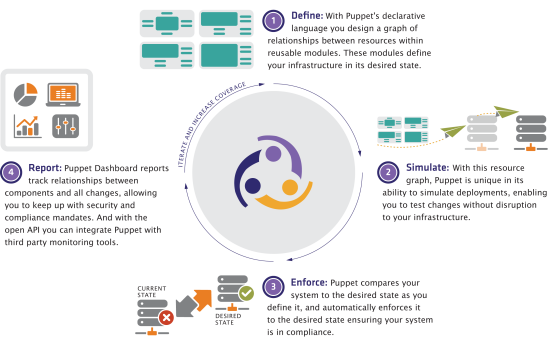
\includegraphics[width=0.7\textwidth]{howpuppetworks}
    \caption{Ciclo de vida de los módulos Puppet}
    \label{fig:howpuppetworks}
\end{figure}

\par El diseño del aprovisionamiento a través de Puppet se basa en módulos. Cada uno de estos módulos se encarga de gestionar la instalación y configuración del componente definido.

\par Que aporta Puppet ? Proporciona un control sobre la instalación de cada herramienta y la configuración asociada por defecto que se define. De esta forma el proceso se instalación se automatiza permitiendo la replicación del mismo, completo o por módulos en diferentes entornos, locales o virtuales. La instalación a partir de módulos ha de definir una cadena de dependencias entre cada uno de ellos de manera que se vayan habilitando funcionalidades e interacciones (Apéndice ~\ref{app:apendice-puppet}).

\par En SidelabCode Stack Puppet es el encargado de gestionar la \emph{instalación y configuración} de cada uno de los componentes mediante módulos Puppet independientes para completar el proceso de instalación (Apéndice ~\ref{app:instalacion-sidelab}) entre 5 y 10 minutos.

%%%%%%%%%%%%%%%%%%%%%%%%%%%%%%%%%%%%%%%%%%%%%%%%%%%%%%%%%%%%%%%%%%%%%%%%%%%%%%%%%%%%%%%%%%%%%%%%%%%%%%%%%%
% Componentes
%%%%%%%%%%%%%%%%%%%%%%%%%%%%%%%%%%%%%%%%%%%%%%%%%%%%%%%%%%%%%%%%%%%%%%%%%%%%%%%%%%%%%%%%%%%%%%%%%%%%%%%%%%

\section{Componentes}
\label{sec:componentes}

\par En este apartado se van a analizar los distintos componentes que integran la Forja SidelabCode Stack y el papel que desempeñan en el funcionamiento del sistema partiendo del esquema en donde se refleja la arquitectura de la Forja SidelabCode ~\ref{fig:scstack-diagram} y la relación que mantienen con las necesidades descritas en el capítulo \nameref{chap:procesos-desarrollo} a la hora de gestionar el proceso \emph{Iterativo e Incremental}.

%%%%%%%%%%%%%%%%%%%%%%%%%%%%%%%%%%%%%%%%%%%%%%%%%%%%%%%%%%%%%%%%%%%%%%%%%%%%%%%%%%%%%%%%%%%%%%%%%%%%%%%%%%
% OpenLDAP
%%%%%%%%%%%%%%%%%%%%%%%%%%%%%%%%%%%%%%%%%%%%%%%%%%%%%%%%%%%%%%%%%%%%%%%%%%%%%%%%%%%%%%%%%%%%%%%%%%%%%%%%%%

\subsection{Usuarios, roles y grupos}
\label{sub:usuarios-roles-grupos}

\par Gestión de usuarios, roles, grupos y proyectos a través de \emph{OpenLDAP}\footnote{OpenLDAP - \url{http://www.openldap.org/}}.

\begin{figure}[H]
    \centering
    
\includegraphics[width=0.3\textwidth]{OpenLDAP-logo}
    \caption{OpenLDAP logo}
    \label{fig:openldap-logo}
\end{figure}

\par SCStack utiliza la tecnología de directorios \emph{LDAP} como sistema de autenticación y de información centralizado de la Forja Software. En dicho servidor de directorios se almacena información relativa a todos los usuarios, proyectos software y repositorios de la Forja. Esta tecnología, además, cuenta con la ventaja de que la mayoría de aplicaciones web con sistemas de autenticación ofrecen interfaces que garantizan una completa integración con directorios LDAP, este es el caso de Redmine, Drupal, Wordpress y el propio servidor web Apache. La implementación de este protocolo en la Forja Sidelab se lleva a cabo mediante un servidor de directorios muy estable y de libre distribución que es OpenLDAP.

\subsection{API OpenLDAP}
\label{sub:api-openldap}

\par Debido a que el directorio LDAP es la estructura de información centralizada de la Forja, cualquier tipo de acción que se quiera realizar sobre el sistema requerirá el acceso por parte de la API a este servicio de directorios, bien para la recuperación de datos en las consultas o para la manipulación de registros a la hora de crear, editar o borrar usuarios o proyectos.

\par Todas las acciones de la Consola de Administración pasan a través de la API que comunica con OpenLDAP dando acceso y generando las distintas autenticaciones en cada una de las herramientas interconectadas basándose en los registros de OpenLDAP como generador y autenticador de credenciales.

% subsection api-openldap (end)

% subsection usuarios-roles-grupos (end)

%%%%%%%%%%%%%%%%%%%%%%%%%%%%%%%%%%%%%%%%%%%%%%%%%%%%%%%%%%%%%%%%%%%%%%%%%%%%%%%%%%%%%%%%%%%%%%%%%%%%%%%%%%
% Gestión de Requisitos - Redmine
%%%%%%%%%%%%%%%%%%%%%%%%%%%%%%%%%%%%%%%%%%%%%%%%%%%%%%%%%%%%%%%%%%%%%%%%%%%%%%%%%%%%%%%%%%%%%%%%%%%%%%%%%%

\subsection{Gestión de Requisitos ITS}
\label{sub:its}

\par La gestión de requisitos en SidelabCode Stack se lleva a cabo a través del Issue Tracking System \emph{Redmine}\footnote{Redmine - \url{http://www.redmine.org/}}.

\begin{figure}[H]
    \centering
    
\includegraphics[width=0.3\textwidth]{redmine}
    \caption{Redmine logo}
    \label{fig:redmine-logo}
\end{figure}

\par Este apartado es el más cuidado e importante en el conjunto de SCStack ya que se trata de la herramienta encargada de centralizar la gestión de \emph{Lista de Control del Proyecto} por cada Iteración. El ITS Redmine es una aplicación web de gestión de proyectos Software multiplataforma desarrollada en \emph{Ruby} a través de \emph{Ruby on Rails}. Por supuesto se trata de una herramienta FLOSS.

\par Redmine proporciona la gestión de tareas (de cualquier tipo; \emph{features, bugs, parches\ldots}) para cada uno de los proyectos creados. Dentro de SCStack se encuentra enlazado a la configuración de usuarios a través de OpenLDAP para la validación y cuenta con una base de datos propia \emph{MySQL}. Un apartado importante ya que esto permite gestionar las migraciones de Redmine de manera rápida, eficiente y fluida de una versión a otra o incluir la información de otro Redmine\footnote{Upgrading Redmine - \url{http://www.redmine.org/projects/redmine/wiki/RedmineUpgrade}} en una nueva instalación de la Forja, únicamente haciendo un backup de la base de datos y algunos directorios clave. Incluso la migración a Redmine desde otros gestores de tareas\footnote{Migrate to Redmine - \url{http://www.redmine.org/projects/redmine/wiki/RedmineMigrate}}.

\par Proporciona una interfaz adaptada para cada proyecto de la forja asociado a un repositorio de código fuente con un visor integrado. Se visualizan los cambios entre distintas versiones del código y comparaciones entre distintas ramas de desarrollo para seguir la evolución del proyecto.

\begin{figure}[H]
    \centering
    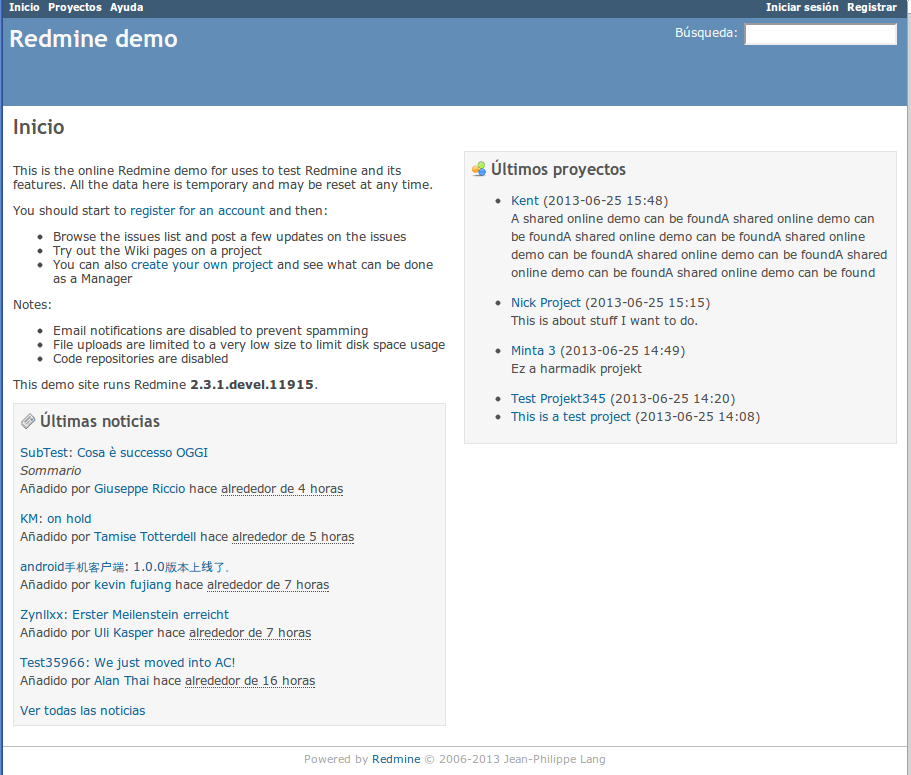
\includegraphics[width=0.7\textwidth]{redmine-demo-landing-page}
    \caption{Redmine página de bienvenida}
    \label{fig:redmine-demo-landing-page}
\end{figure}

\par Dentro del proceso Iterativo e Incremental como herramientas nos proporciona informes de seguimiento de actividad dinámicos (\emph{día, persona, proyecto\ldots}), un \emph{Wiki} para la documentación y una página de noticias.

\par Es la interfaz web de entrada al proyecto para los desarrolladores, por ello es la parte más importante y en donde se centran gran parte de los esfuerzos para la fluidez y la importancia que tiene la misma.

\par Por otra parte Redmine proporciona una API Rest para facilitar la interoperabilidad entre los distintos componentes. Esta API se maneja a través de la capa de negocio de la Consola de Administración de SCStack para así a través del API se registren en Redmine los usuarios, proyectos y grupos con sus respectivos permisos partiendo de los valores introducidos a través de la Consola de Administración. De esta forma, Redmine pasa a gestionar a través de su BBDD MySQL los usuarios y proyectos después que se hayan autenticado a través de OpenLDAP para así cargar la configuración obtenida de su BBDD.

\par Las operaciones de gestión administrativa en Redmine permanecen desactivadas, de modo que ningún administrador de proyectos puede añadir ni borrar miembros de sus proyectos, tampoco pueden crearse ni borrarse usuarios o proyectos, etc. \emph{Obligando} así que todas las operaciones de gestión de la Forja se lleven a cabo desde el Software diseñado específicamente para ello, la Consola de Administración, garantizando así la consistencia.

\subsection{Plugins}
\label{sub:redmine-plugins}

\par A la hora de aplicar el desarrollo Iterativo e Incremental se intenta incrementar la eficacia, la visibilidad, la rapidez y la comprensión del proceso de desarrollo. Por eso se han utilizado distintos plugins para Redmine que ayudan a la comprensión y agilizan el proceso Iterativo e Incremental para los usuarios (desarrolladores, gestores, etc\ldots) a través del plugin FLOSS \emph{Backlogs}\footnote{Redmine Backlogs - \url{http://www.redminebacklogs.net/}}.

\par \emph{Backlogs} aporta una gestión visual en modo tablón de las Iteraciones activas en el proceso. Gestiona 'manualmente' a través de \emph{Drag and Drop} la organización de las tareas del proyecto y agiliza la comprensión del estado de la iteración, proyecto, desarrollo en sí, en un sólo vistazo ~\ref{fig:backlogs-plugin}.

\begin{figure}[H]
    \centering
    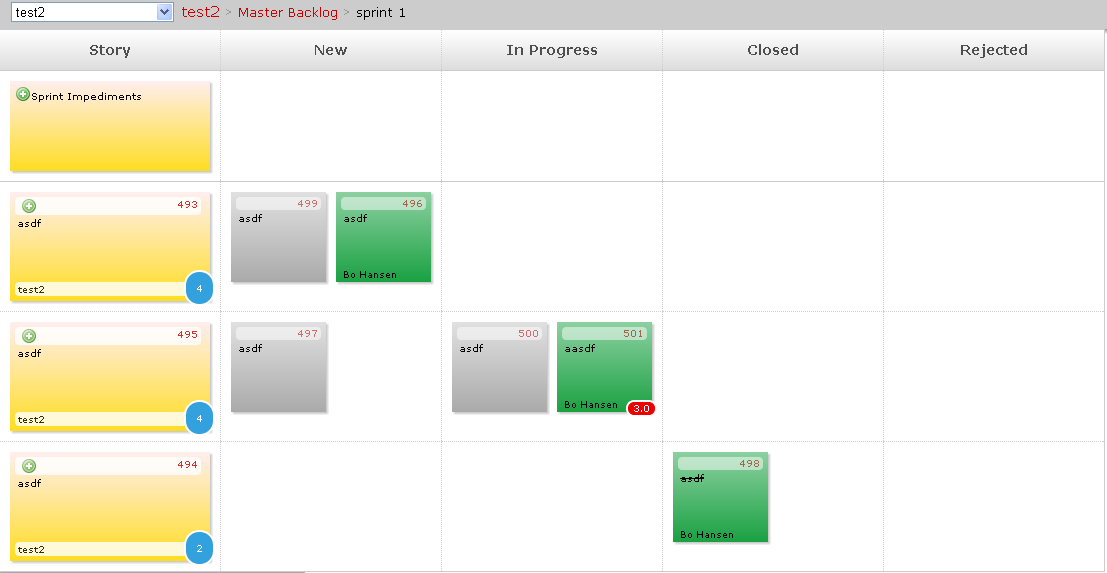
\includegraphics[width=0.7\textwidth]{backlogs-plugin}
    \caption{Redmine Backlogs plugin: tareas Redmine agrupadas por estados dentro de una historia de usuario.}
    \label{fig:backlogs-plugin}
\end{figure}

\par Otro apartado importante en el desarrollo Iterativo e Incremental es la gestión de la documentación, en este caso Redmine nos proporciona una Wiki por cada proyecto. Una Wiki es una herramienta para la documentación colaborativa que mantiene su histórico de cambios (asociados a usuario y tiempo) y que mediante el lenguaje de marcado wiki desde el cual se exportan a distintos formatos como: \emph{html, pdf, etc}, a un coste de recursos bajo ya que se trata de texto plano. El caso más famoso del uso de Wikis como documentación colaborativa es la \emph{Wikipedia}\footnote{Wikipedia - \url{http://www.wikipedia.org}}.

% subsection redmine-plugins (end)

% subsection its (end)

%%%%%%%%%%%%%%%%%%%%%%%%%%%%%%%%%%%%%%%%%%%%%%%%%%%%%%%%%%%%%%%%%%%%%%%%%%%%%%%%%%%%%%%%%%%%%%%%%%%%%%%%%%
% Repositorios de Código
%%%%%%%%%%%%%%%%%%%%%%%%%%%%%%%%%%%%%%%%%%%%%%%%%%%%%%%%%%%%%%%%%%%%%%%%%%%%%%%%%%%%%%%%%%%%%%%%%%%%%%%%%%

\subsection{Repositorios de Código}
\label{sub:repositorios}

\par Los repositorios de código (VCS) son los encargados de gestionar el ciclo de vida del código fuente como hemos visto en el apartado de Código versionado~\ref{sec:codigo-versionado} y existen dos tipos: centralizados y distribuidos. Para el proceso de desarrollo Iterativo e Incremental hemos seleccionado el repositorio distribuido \emph{Git}\footnote{Git - \url{http://git-scm.com/}}.

\begin{figure}[H]
    \centering
    
\includegraphics[width=0.3\textwidth]{git-logo}
    \caption{Git SCM Logo}
    \label{fig:git-scm-logo}
\end{figure}

\par Atendiendo a los requerimientos del proceso:

\begin{quote}
    \emph{El desarrollo de la solución se adapta al uso del Repositorio distribuido, ya que éste aporta una flexibilidad para la gestión de bifurcaciones del código que en un repositorio centralizado no tenemos fácilmente}
\end{quote}

\par En el proceso Iterativo e Incremental abundan las ramificaciones del código en el repositorio debido a ello se opta por la elección del repositorio distribuido Git en pro del repositorio centralizado SVN, que también se incluye en la Forja SCStack. Las ramificaciones, la cantidad de fusiones entre ramas~\cite{featurebranch}, entornos de desarrollo sumando la facilidad, agilidad y el bajo coste en Git nos proporcionan la herramienta adecuada para la gestión del código fuente en SCStack.

\par En el repositorio Git no se guardan diferencias se guardan snapshots en comparación con Subversion.

\begin{figure}[H]
    \centering
    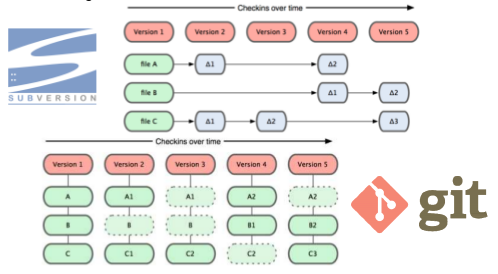
\includegraphics[width=0.7\textwidth]{svn-git-comparison}
    \caption{Comparación de incrementos entre SVN (completo) y Git (incrementos en archivos)}
    \label{fig:svn-git-comparison}
\end{figure}

\begin{quotation}
    \emph{For example the Mozilla repository is reported to be almost 12 Gb when stored in SVN using the fsfs backend. Previously, the fsfs backend also required over 240,000 files in one directory to record all 240,000 commits made over the 10 year project history. This was fixed in SVN 1.5, where every 1000 revisions are placed in a separate directory. The exact same history is stored in Git by only two files totaling just over 420 Mb. This means that SVN requires 30x the disk space to store the same history}\footnote{Git Svn Comparison Smaller Space Requirements - \url{https://git.wiki.kernel.org/index.php/GitSvnComparison\#Smaller\_Space\_Requirements}}
\end{quotation}

\par Asociada a cada Iteración se ha de gestionar la viabilidad de una rama del repositorio. En esta rama se trabaja con respecto a las tareas a desarrollar para la iteración. Se hacen las pruebas necesarias para cada desarrollo para después integrar la solución en la rama principal y así crear una nueva versión del proyecto. 

\par La ramificación del desarrollo permite gestionar por iteraciones incrementales aisladas en una nueva rama, de esta forma, el contenido de la rama principal es fiable, ya que para añadir contenido a la rama ha tenido que pasar una iteración nueva y el proceso de desarrollo que conlleva; planificación, test, implementación e integración. El resultado está altamente controlado y distribuido en base a módulos para poder acotar posibles errores posteriores o revertir cambios a través de un proceso minuciosamente controlado.

\subsubsection{Integridad}
\label{subs:git-integridad}

\par Los commits se identifican por un \texttt{hash sha1}

\begin{itemize}
    \item \texttt{Svn}: \emph{rev 33}
    \item \texttt{Git}: \emph{d025a7b3217f05110ebbf48065b8d02a0ad22ae3}
\end{itemize}

\par O más amigablemente: \emph{d025a7b}

\par Los ficheros también se identifican por su sha1 de esta forma si un fichero se corrompe durante la transmisión por la red se detecta inmediatamente

\subsubsection{Los 3 estados}
\label{subs:git-3-estados}

\par Los ficheros en Git pueden estar en tres estados:

\begin{itemize}
    \item \texttt{Modificado}: el fichero ha cambiado desde el último checkout
    \item \texttt{Staged}: un fichero modificado ha sido marcado para ser añadido en el próximo commit
    \item \texttt{Committed}: el fichero se encuentra en la base de datos de git
\end{itemize}

\par Hay un 4º estado: \textbf{untracked}.

\subsubsection{Las 3 áreas de un proyecto git}
\label{subs:git-3-areas}

\begin{enumerate}
    \item El directorio git (git directory):
        \begin{itemize}
            \item Contiene los metadatos y la base de datos de git
            \item Es lo que se copia cuando se clona un repositorio
            \item Normalmente es una carpeta .git en algún directorio
        \end{itemize}
    \item La carpeta de trabajo (working directory):
        \begin{itemize}
            \item Es un checkout de una versión específica del proyecto
            \item Se extrae del directorio git
            \item Es el espacio donde modificamos los ficheros
        \end{itemize}
    \item Staging area:
        \begin{itemize}
            \item Fichero en el directorio git que indica qué cambios van en el próximo commit
        \end{itemize}
\end{enumerate}

\begin{figure}[H]
    \centering
    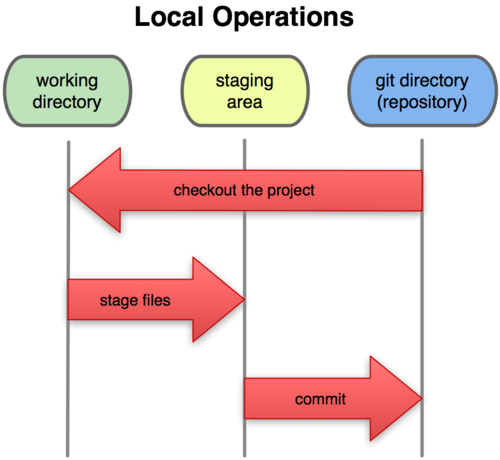
\includegraphics[width=0.7\textwidth]{git-3-areas}
    \caption{Tres áreas en Git}
    \label{fig:git-3-areas}
\end{figure}

\subsubsection{La identidad}
\label{subs:git-identidad}

\par Git necesita conocer algunos datos del desarrollador (aparecen en los commits para identificar al autor)

\begin{itemize}
    \item Nombre
    \item Email
\end{itemize}

\par Si no están correctamente configurados pueden aparecer varios problemas:

\begin{itemize}
    \item Los commits \textbf{fallan} porque el usuario no está autorizado
    \item Commits del mismo usuario \emph{'físico'} \textbf{no son considerados como del mismo usuario} porque el nombre \emph{'lógico'} cambia.
\end{itemize}

\par Por lo que se ha de tener muy en cuenta este apartado y configurar correctamente en el archivo.

% subsection repositorios (end)

\subsection{Revisión de Código}
\label{sub:gerrit}

\par La gestión del repositorio Git está orientada a través de la herramienta \emph{Gerrit}\footnote{\url{http://code.google.com/p/gerrit/}}.

\begin{figure}[H]
    \centering
    
\includegraphics[width=0.3\textwidth]{gerrit-diffy}
    \caption{Gerrit Kunfu Review Cuckoo}
    \label{fig:gerrit-logo}
\end{figure}

\par Gerrit es una herramienta de revisión de código basada en web. Facilita el control online de las revisiones de código para los proyectos a través de la herramienta Git.

\par Gestiona la autenticación y la gestión de permisos, roles y grupos para cada uno de los repositorios existentes a través de una interfaz ligera. Un punto a destacar es la orientación hacia un repositorio centralizado de Git, es decir, el control de código se centraliza en un repositorio para la integración dependiente de los repositorios de los desarrolladores\footnote{Git Flujo de trabajo centralizado - \url{http://git-scm.com/book/es/Git-en-entornos-distribuidos-Flujos-de-trabajo-distribuidos\#Flujo-de-trabajo-centralizado}}.

\begin{figure}[H]
    \centering
    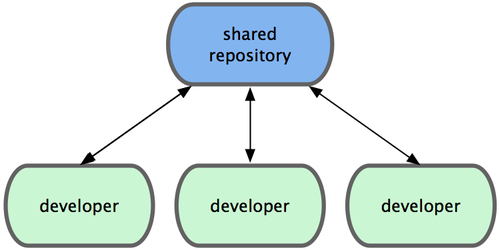
\includegraphics[width=0.7\textwidth]{git-centralizado}
    \caption{Git: Flujo de trabajo centralizado}
    \label{fig:git-centralizado}
\end{figure}

\par Centralizar la rama principal del proyecto en el repositorio descentralizado casa perfectamente con el proceso Iterativo e Incremental ya que a cada iteración cerrada añadimos los cambios a la rama estable del proyecto desarrollado centralizando el código a empaquetar para convertir en la solución final, incremento a incremento.

\par La configuración viene a través del API de SCStack y una consola interactiva SSH\footnote{Gerrit Command Line Tools - \url{http://gerrit.googlecode.com/svn/documentation/2.0.34/cmd-index.html}} que proporciona Gerrit. En SCStack esta función recae sobre los valores obtenidos del servidor \emph{OpenLDAP} a partir de los datos introducidos en la Consola de Administración a la hora de gestionar la creación de un proyecto y el grupo de usuarios asociados al proyecto siguiendo el flujo de datos centralizado a través de la API Rest central. La creación del proyecto, la gestión de usuarios y permisos sobre el repositorio Git creado.

\par Este procedimiento se encapsula a través del envío de órdenes a la consola a través del API habiendo configurado la autenticación a través de un conjunto de clave SSH en la instalación de SCStack.

% subsection gerrit (end)

%%%%%%%%%%%%%%%%%%%%%%%%%%%%%%%%%%%%%%%%%%%%%%%%%%%%%%%%%%%%%%%%%%%%%%%%%%%%%%%%%%%%%%%%%%%%%%%%%%%%%%%%%%
% Integración Continua
%%%%%%%%%%%%%%%%%%%%%%%%%%%%%%%%%%%%%%%%%%%%%%%%%%%%%%%%%%%%%%%%%%%%%%%%%%%%%%%%%%%%%%%%%%%%%%%%%%%%%%%%%%

\subsection{Integración Continua}
\label{sub:ci-jenkins}

\par  La integración continua dentro del proceso de desarrollo Iterativo e Incremental es la encargada de agilizar la comunicación entre los distintos actores involucrados. Evalúa la evolución de la solución y provee una respuesta firme y profesional para afianzar los resultados de cada incremento.

\begin{figure}[H]
    \centering
    
\includegraphics[width=0.3\textwidth]{jenkins}
    \caption{Jenkins CI Logo}
    \label{fig:jenkins-logo}
\end{figure}


\par En este aspecto, la herramienta que SCStack necesita es un gestor de integración continua como \emph{Jenkins-CI}\footnote{Jenkins-CI - \url{http://jenkins-ci.org}}:

\begin{quote}
    \emph{In a nutshell Jenkins CI is the leading open-source continuous integration server. Built with Java, it provides over 400 plugins to support building and testing virtually any project.}
\end{quote}

\par Jenkins-CI\footnote{Meet Jenkins-CI - \url{https://wiki.jenkins-ci.org/display/JENKINS/Meet+Jenkins}} proporciona la integración de la integración continua (valga la redundancia) en el proceso de desarrollo de software de una forma modular e interoperable. No se trata de un servidor intrusivo ni para el proceso de desarrollo ni para el desarrollador en si.

\par En este aspecto SCStack incluye el módulo de Jenkins-CI en la instalación para facilitar el trabajo de las pruebas, integración y generación de versiones mediante la virtualización de escenarios más cercanos al sistema de producción. Des esta forma se perfila mejor el rendimiento, la replicación de errores y el control de la evolución del código fuente. Dentro del desarrollo, el código fuente es el centro de la calidad y debido a esta afirmación, se necesita un servidor de CI adaptado al proceso de desarrollo.

\begin{itemize}
	\item Tags.
	\item Construir las versiones vivas.
	\item Branches de releases.
	\item Desplegar una versión específica con un clic.
\end{itemize}

\par Jenkins-CI se instala integrado en el marco de trabajo SCStack interoperando entre el repositorio de código fuente Git, la herramienta de gestión Gerrit y el despliegue de los tests en servidores como Apache o Tomcat dependiendo del producto final (esto no tiene nada que ver con el desarrollo, sería un requisito del proyecto). Jenkins-CI mantiene diferentes versiones vivas a la vez en el repositorio del proyecto para cumplir con los objetivos:

\begin{itemize}
	\item Asegurar la calidad.
	\item Hacer el despliegue ágil.
	\item Minimizar el riesgo.
\end{itemize}

\par Jenkins-CI trabaja en base a \emph{Jobs}. Un Job en Jenkins-CI describe el proceso de integración, pruebas o despliegue que va a ejecutarse cuando se cumpla un requisito definido o manualmente. La integración de las distintas ramas de desarrollo en cada iteración en el ciclo de vida~\ref{fig:simple-lifecycle} las gestiona Jenkins-CI a través de los Jobs definidos:

\begin{itemize}
	\item Jobs de \emph{integración}.
	    \begin{itemize}
        	\item Descargan el código del repositorio Git.
        	\item Construyen.
        	\item Pasan tests.
        	\item Despliegan la versión construida en "local".
        \end{itemize}
	\item Jobs de \emph{release}.
	    \begin{itemize}
        	\item Realizan los pasos anteriores y además.
        	\item Tag si los tests pasaron.
        	\item Push del tag al repositorio remoto.
        \end{itemize}
	\item Jobs de \emph{despliegue}.
	    \begin{itemize}
        	\item Descargan el binario del repositorio de binarios
        	\item Desplegar en un servidor de aplicaciones.
        \end{itemize}
\end{itemize}

\begin{figure}[H]
    \centering
    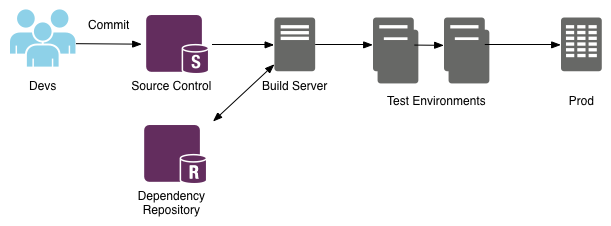
\includegraphics[width=0.7\textwidth]{simple-lifecycle}
    \caption{Ciclo de vida Jenkins CI}
    \label{fig:simple-lifecycle}
\end{figure}

\par Dentro de la forja SCStack se configura el uso de Jenkins-CI a partir de usuarios dedicados a la gestión de jobs. Se plantean tres opciones:

\begin{itemize}
	\item \textbf{Opción I}: Un usuario \emph{jenkinsci} con acceso de \emph{lectura/escritura} a \emph{todos} los repositorios.
        \begin{itemize}

        	\item \emph{Pros}; Simplicidad: sólo hay que gestionar un usuario. Una \emph{única} clave ssh \emph{/home/tomcat/.ssh/id\_rsa.pub}.
        	\item \emph{Contras}; Un usuario para dominarlos a todos. Cualquier error en un job para el proyecto \emph{X} puede afectar a los repositorios del proyecto \emph{Y}.
        \end{itemize}

	\item \textbf{Opción II}: Un usuario @jenkinsci@ con acceso de \emph{lectura/escritura} a todos los repositorios y  otro \emph{jenkinsci\_read} con acceso sólo de lectura	
        \begin{itemize}
        	\item \emph{Pros}; Sólo hay que gestionar \emph{dos usuarios}: basta con asociarlos a \emph{todos} los proyectos.
        	\item \emph{Contras}; Seguimos teniendo un usuario para dominarlos a todo: jenkinsci. Cualquier error en un job para el proyecto \emph{X} puede afectar a los repositorios del proyecto \emph{Y}. Hay que gestionar dos claves ssh. No es trivial.
        \end{itemize}

	\item \textbf{Opción III}: Un \emph{usuario por proyecto} para integración continua.
        \begin{itemize}
        	\item \emph{Pros}; El usuario de ci de un proyecto no tiene acceso a los repositorios de otro proyecto.
        	\item \emph{Contras}; Hay que gestionar múltiples \emph{claves ssh}.
        \end{itemize}

\end{itemize}

\par Se decide utilizar un usuario por proyecto definida en la \textbf{tercera opción}, después de haber evaluado las distintas opciones.
 
\par La gestión de los usuarios se gestiona a través de la consola de administración de SCStack. De esta manera la herramienta nos aporta una vía única de entrada dotando de la funcionalidad específica para distintos estados del proceso de desarrollo nada intrusivos en el desarrollo del proyecto. Separando a través del API de SCStack la gestión y partiendo de los roles/usuarios/grupos definidos como base en OpenLDAP.

\par El repositorio remoto debería contener versiones más o menos estables y distinguidas para el desarrollo por ramas establecido el proceso:

\begin{itemize}
	\item \textbf{Develop}: Pueden fallar algunos tests, no es problema.

	\item \textbf{Release-X}: Los tests deberían pasar, eventualmente se podrían desactivar.
	
	\item \textbf{Nightly builds}: Construcciones que comprueban la \emph{'salud'} del proyecto. Se hacen sobre los branches \emph{development} y \emph{release-X} (siendo X la versión más reciente).

    \begin{itemize}
	    \item Se ejecutan los tests.
	    \item Se despliegan dos versiones por cada rama: \texttt{Limpia}: una bbdd nueva y \texttt{Migración}: con actualización de bbdd ya existente sobre la bbdd que ya hubiera para ese despliegue.
    \end{itemize}

	\item \textbf{Preproducción}: Las versiones que van a preproducción son aquellas de las que se ha hecho \texttt{tag}: 
	\begin{itemize}
	    \item Pasan los tests.
	    \item El entorno de pre puede estar en \emph{local} o en \emph{Remoto}.
	    \item Se despliegan dos versiones: \texttt{Limpia} y \texttt{Migración}.
    \end{itemize}

	\item \textbf{Producción}: Las versiones que van a producción son aquellas de las que se ha hecho \texttt{tag}.
	\begin{itemize}
	    \item Pasan los tests.
	    \item El despliegue se realiza en \emph{Remoto}.
	    \item Se despliegan dos versiones: \texttt{Limpia} y \texttt{Migración}.
    \end{itemize}

\end{itemize}

\begin{figure}[H]
    \centering
    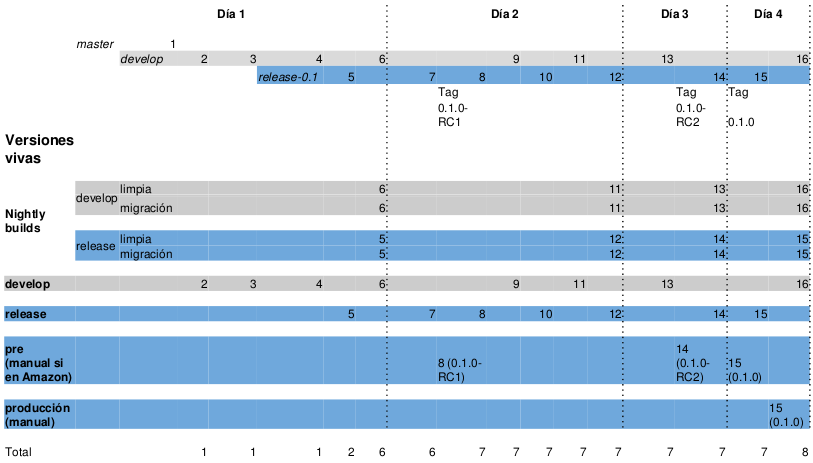
\includegraphics[width=0.7\textwidth]{diagrama-integracion-continua}
    \caption{Integración Continua de versiones a partir de distintas ramas}
    \label{fig:diagrama-integracion-continua}
\end{figure}

% subsection ci-jenkins (end)

%%%%%%%%%%%%%%%%%%%%%%%%%%%%%%%%%%%%%%%%%%%%%%%%%%%%%%%%%%%%%%%%%%%%%%%%%%%%%%%%%%%%%%%%%%%%%%%%%%%%%%%%%%
% Gestión de distribuciones y dependencias
%%%%%%%%%%%%%%%%%%%%%%%%%%%%%%%%%%%%%%%%%%%%%%%%%%%%%%%%%%%%%%%%%%%%%%%%%%%%%%%%%%%%%%%%%%%%%%%%%%%%%%%%%%

\subsection{Gestión de distribuciones y dependencias}
\label{sub:distribuciones-dependencias}

\par Gestión de recursos compartidos, comunicación segura a través de \emph{OpenSSH} y gestión de dependencias y distribuciones a través de \emph{Archiva} como repositorio \emph{Maven}.

\subsubsection{OpenSSH}
\label{ssub:openssh}

\par \emph{OpenSSH}\footnote{\url{http://www.openssh.org/}} es un conjunto de aplicaciones de libre distribución que permiten realizar comunicaciones cifradas a través de la red usando el protocolo SSH.

\begin{figure}[H]
    \centering
    
\includegraphics[width=0.3\textwidth]{openssh_logo}
    \caption{OpenSSH logo}
    \label{fig:openssh_logo}
\end{figure}

\par La función fundamental que brinda este protocolo a la Forja Software consiste en garantizar que los usuarios de los distintos proyectos puedan acceder, por ejemplo a través de SFTP\footnote{\url{http://en.wikipedia.org/wiki/SFTP}} o Secure Shell \emph{SSH}\footnote{\url{http://en.wikipedia.org/wiki/Secure\_Shell}}, a las carpetas privadas y públicas de los proyectos en los cuales participan, a través de una conexión cifrada, y gestionar sus ficheros de una forma sencilla, ágil y segura.

% subsubsection openssh (end)

\subsubsection{Archiva}
\label{ssub:archiva}

\par \emph{Archiva}\footnote{\url{http://archiva.apache.org/index.cgi}} es una aplicación FLOSS para la gestión de repositorios de artefactos de construcción, desarrollado por \emph{Apache Software Foundation}. Este el compañero perfecto para herramientas de construcción como Maven.

\begin{figure}[H]
    \centering
    
\includegraphics[width=0.3\textwidth]{apache-archiva-logo}
    \caption{Apache Archiva logo}
    \label{fi:apache-archiva}
\end{figure}

\par Entre las funcionalidades que podemos destacar de esta herramienta están, el proxy para repositorio remoto (reduce el tráfico de red en equipos de trabajo), la gestión del control de acceso a los repositorios definidos, la construcción de artefactos de almacenamiento y, la gestión y mantenimiento de repositorios Maven facilitando la indexación, búsquedas, informes, estadísticas.

\par Posee una interfaz web sencilla de configurar en la que publica el contenido del repositorio Maven accesible a los usuarios autenticados. Además de el acceso al repositorio Maven habiendo configurado en los proyectos de desarrollo la url en la que está publicado:

\lstset{style=xmlbasico}
\begin{lstlisting}[frame=trbl]
<project>
  <!-- omitted xml -->
  <distributionManagement>
    <repository>
      <id>archiva.internal</id>
      <name>Internal Release Repository</name>
      <url>http://reposerver.mycompany.com:8080/archiva/repository/internal/</url>
    </repository>
    <snapshotRepository>
      <id>archiva.snapshots</id>
      <name>Internal Snapshot Repository</name>
      <url>http://reposerver.mycompany.com:8080/archiva/repository/snapshots/</url>
    </snapshotRepository>
  </distributionManagement>
  <!-- omitted xml -->
</project>
\end{lstlisting}

\par El uso de Archiva como gestor de dependencias Maven puede ser público y/o privado dependiendo del repositorio que se cree. De esta forma los equipos de desarrolladores automatizan y centralizan las descargas de las dependencias (librerías) a través de Archiva dentro de la red local, disminuyendo el tráfico de red y agilizando la puesta en marcha de proyectos y los jobs de CI, reduciendo el consumo.

% subsubsection archiva (end)

% subsection distribuciones-dependencias (end)

% subsection componentes (end)

%%%%%%%%%%%%%%%%%%%%%%%%%%%%%%%%%%%%%%%%%%%%%%%%%%%%%%%%%%%%%%%%%%%%%%%%%%%%%%%%%%%%%%%%%%%%%%%%%%%%%%%%%%
% Desarrollo Eclipse y Maven
%%%%%%%%%%%%%%%%%%%%%%%%%%%%%%%%%%%%%%%%%%%%%%%%%%%%%%%%%%%%%%%%%%%%%%%%%%%%%%%%%%%%%%%%%%%%%%%%%%%%%%%%%%

\subsection{Desarrollador: Eclipse y Maven}
\label{sub:eclipse-mvn-tdd}

\par El entorno de desarrollo para el desarrollador en el que se integra el proceso Iterativo e Incremental consta de dos herramientas y un concepto.

\par El IDE \emph{Integrated Development Environment} a utilizar es Eclipse, concretamente la distribución del framework Spring \emph{Eclipse STS}\footnote{Eclipse STS - \url{http://www.springsource.org/sts}}. 

\begin{figure}[H]
    \centering
    
\includegraphics[width=0.3\textwidth]{STS}
    \caption{Spring Tool Suite logo}
    \label{fig:sts}
\end{figure}

\par STS otorga y proporciona un conjunto de herramientas preparadas para trabajar con los componentes de STStack: Redmine, Git, Gerrit, Jenkins, Apache, OpenLDAP, Maven. Se basa en unan distribución de Eclipse orientada al desarrollo para trabajar con diferentes componentes externos facilitando la puesta a punto para empezar a desarrollar.

\par Esta distribución incluye la gestión de un proyecto a través \emph{Maven}\footnote{Apache Maven - \url{http://maven.apache.org/}}. Maven es un Software de gestión de proyectos basado en la definición del proyecto POM (Project Object Model). Es el encargado de compilar, ejecutar test, desplegar, gestionar las dependencias (locales y remotas) y generar distribuciones a partir de una configuración definida.

\begin{figure}[H]
    \centering
    
\includegraphics[width=0.3\textwidth]{maven}
    \caption{Maven logo}
    \label{fig:maven-logo}
\end{figure}

\par Esta herramienta se integra en el ciclo de vida del Software para automatizar los procesos tediosos manuales, proveer una estructura básica inicial a los proyectos (iteración 0) para ir incrementando iteración tras iteración a través de los arquetipos.

\par Incorpora componentes en la instalación por defecto para facilitar el trabajo del desarrollador con la forja SCSTack:

\begin{itemize}
	\item \emph{Egit} - Plugin de Eclipse para trabajar con repositorios Git - \url{http://www.eclipse.org/egit/}.
	\item \emph{Mylyn} - Plugin para gestionar las tareas del ITS, en este caso Redmine, a través de la interfaz de Eclipse. Automatizando las pruebas, grabando sesiones de trabajo e incluso compartirlas para poder reproducir un procedimiento en otro sistema - \url{http://www.eclipse.org/mylyn/}
	\item \emph{Maven} - Plugin \emph{2eclipse} para la gestión de proyectos Maven a través de su ciclo de vida. Ayuda a facilitar la configuración de los builds a través de los pom de Maven. Genera esqueletos de proyectos a través de los arquetipos de una forma intuitiva - \url{http://www.sonatype.org/m2eclipse}
\end{itemize}

\par A través de Maven y Eclipse se definen las líneas del desarrollo de cada iteración facilitando el diseño TDD~\ref{sub:tdd} a través de una sencilla configuración. El esqueleto de los proyectos Maven proporciona unas sencillas guías estándar para el desarrollo de proyectos de Software. Esta agrupación de funcionalidades se reutiliza en Jenkins-CI a través de los \emph{jobs} de Maven para así poder replicar cualquier entorno durante la integración continua partiendo de una base robusta.

% subsection eclipse-mvn-tdd (end)

%%%%%%%%%%%%%%%%%%%%%%%%%%%%%%%%%%%%%%%%%%%%%%%%%%%%%%%%%%%%%%%%%%%%%%%%%%%%%%%%%%%%%%%%%%%%%%%%%%%%%%%%%%
% Pruebas y Validación
%%%%%%%%%%%%%%%%%%%%%%%%%%%%%%%%%%%%%%%%%%%%%%%%%%%%%%%%%%%%%%%%%%%%%%%%%%%%%%%%%%%%%%%%%%%%%%%%%%%%%%%%%%

\section{Pruebas y Validación}
\label{sec:pruebas-validacion}

\par Todo proyecto de software necesita ser probado para comprobar que funcione correctamente si existen fallos para así poder atajarlos sin que las sorpresas aparezcan.

\par El lenguaje utilizado para el desarrollo del API del proyecto ha sido \emph{Java}.

\begin{figure}[H]
    \centering
    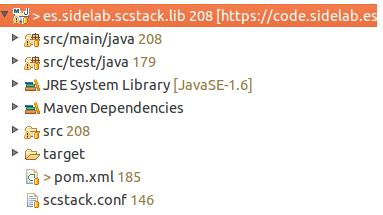
\includegraphics[width=0.5\textwidth]{sidelabcodestack-api-lib}
    \caption{SidelabCode Stack Librería API}
    \label{fig:sidelabcodestack-api-lib}
\end{figure}

\par Para las pruebas del proyecto de la generación del API se ha utilizado en framework \emph{JUnit}\footnote{JUnit - \url{http://junit.org/}}. La cobertura de tests del proyecto en JUnit no es muy halagüeña ya que es del 3,5\%~\ref{fig:sidelabcodestack-sonar} pero en su defensa se puede justificar debido a que se trata de una librería que accede a APIs de terceros. Las APIs o librerías de terceros no han de desarrollar test unitarios sino test test de aprendizaje por lo que no son tan útiles~\cite{clean-code}.

\par Por parte de la publicación del API como servicio Web REST se ha utilizado framework Restlet pero en este caso vemos que la cobertura de test es del 0\%~\ref{fig:sidelabcodestack-sonar-rest-service}. A partir de un proyecto nuevo y dependiente que utiliza la libraría API para publicarla como Servicio Web REST ofreciendo las funcionalidades a la Consola de Administración de la Forja.

\par He utilizado la herramienta \emph{SonarQube}\footnote{SonarQube - \url{http://www.sonarqube.org/}} para obtener una visión más empírica del estado de la cobertura del proyecto. Utilizando las reglas básicas para poder fijarnos en la cantidad de pruebas definidas para SidelabCode Stack \emph{API Lib}~\ref{fig:sidelabcodestack-sonar} y \emph{REST Services}~\ref{fig:sidelabcodestack-sonar-rest-service} ya que para obtener este dato no hace falta un gran refinamiento en la configuración.

\begin{figure}[H]
    \centering
    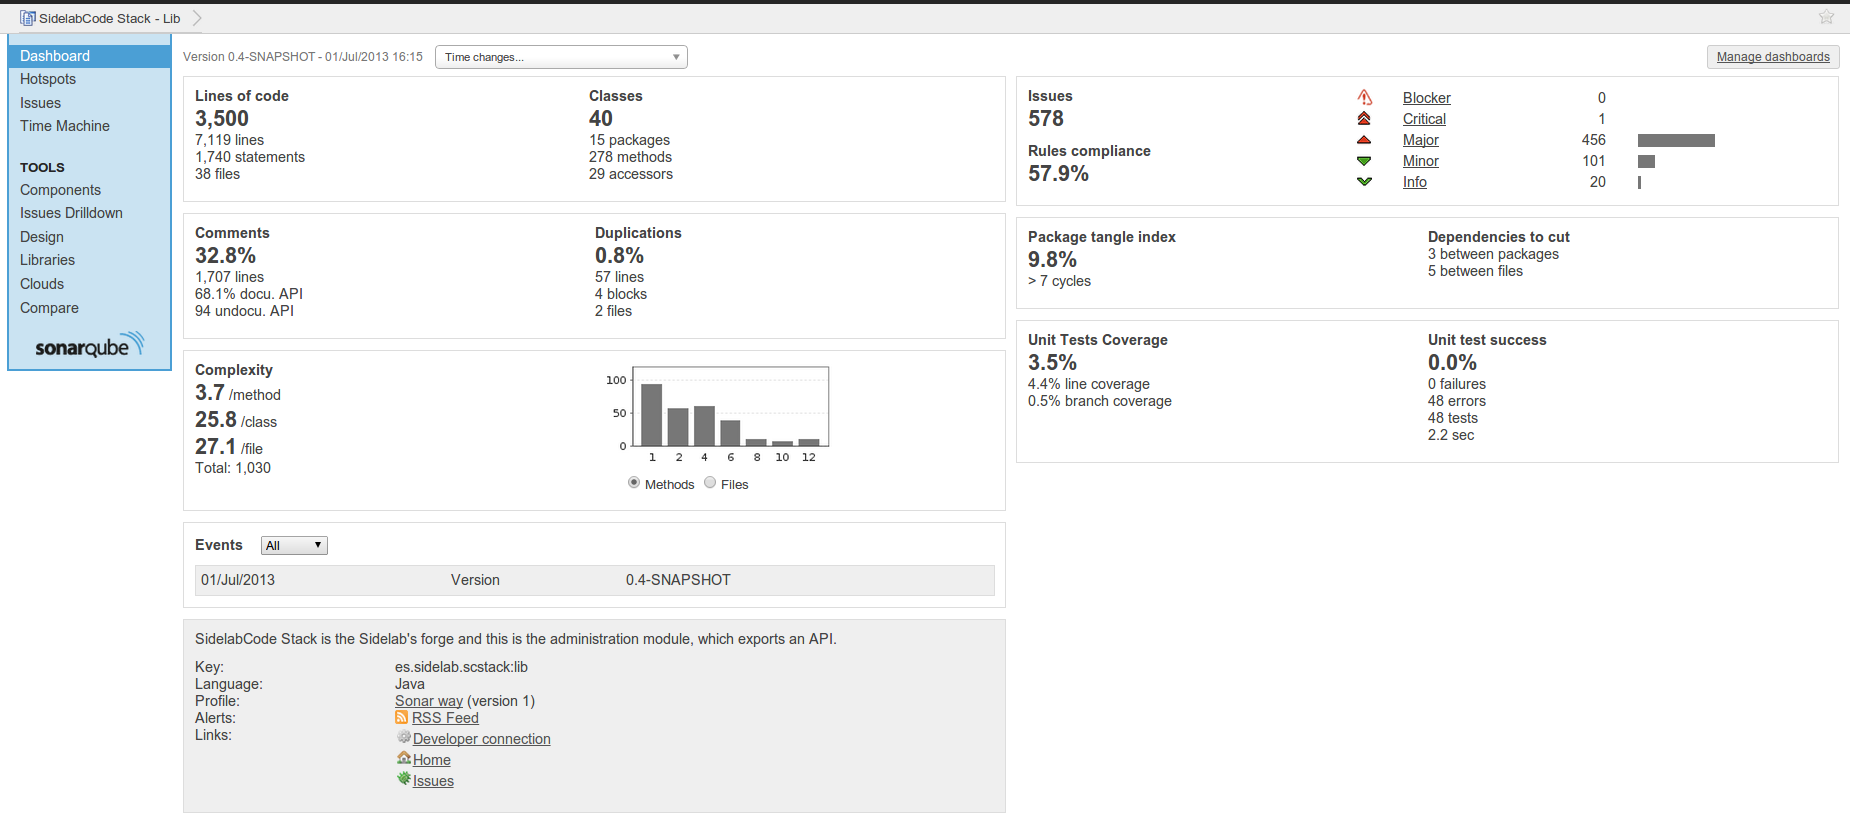
\includegraphics[width=\textwidth]{sidelabcodestack-sonar}
    \caption{SidelabCode Stack API lib Análisis de cobertura con Sonar}
    \label{fig:sidelabcodestack-sonar}
\end{figure}

\begin{figure}[H]
    \centering
    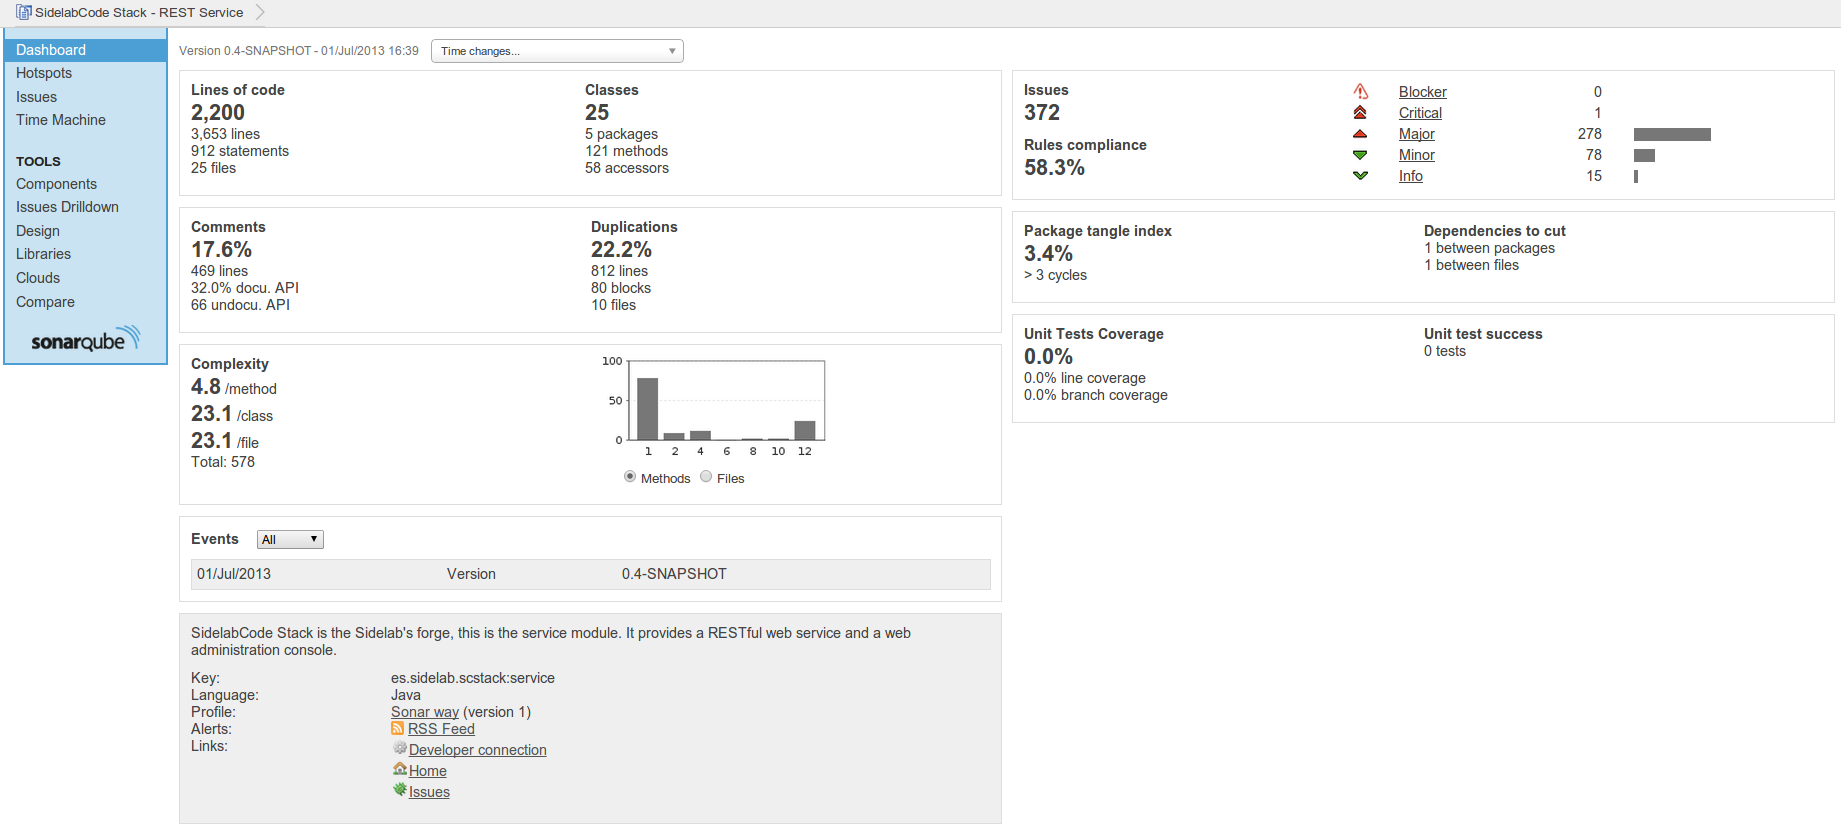
\includegraphics[width=\textwidth]{sidelabcodestack-sonar-rest-service}
    \caption{SidelabCode Stack REST Service Análisis de cobertura con Sonar}
    \label{fig:sidelabcodestack-sonar-rest-service}
\end{figure}

\par El an\'alisis del seguimiento a trav\'es de SonarQube tiene como objetivo mostrar el estado del proyecto y definir el horizonte al que se quiere llegar:

\begin{itemize}
	\item Incrementar la calidad dentro de un rango. Partiendo de una base como primer an\'alisis.
	\item Controlar el avance la de la calidad por iteraciones.
	\item Mejorar el desarrollo.
\end{itemize}

\subsection{Pruebas instalación}
\label{sub:pruebas-instalacion}

\par Las pruebas más importantes en el proceso de desarrollo de la forja SidelabCodeStack han sido las de instalación y configuración de la forja que es donde se encuentra el valor del proyecto. 

\par Previamente a la versión de la forja 0.2 la instalación se ejecutaba a partir de un instalador Java y en consecuencia las pruebas y la replicación de los errores en diferentes entornos acarreaban un trabajo que no podía asumirse con sencillez. A partir de la citada versión (0.2) se introdujo Puppet como herramienta de aprovisionamiento y configuración de los distintos módulos que componen la forja. Este framework ofrece un nuevo camino dentro de las pruebas en el proceso de desarrollo, \emph{la virtualización de las instalaciones}. Puppet nos proporciona un seguimiento completo de la instalación paso a paso a partir de la configuración definida en el proceso. Facilita la ejecución de la instalación de forja en entornos virtuales y seguros para poder asegurar el correcto funcionamiento y descubrir los posibles errores.

\begin{figure}[H]
    \centering
    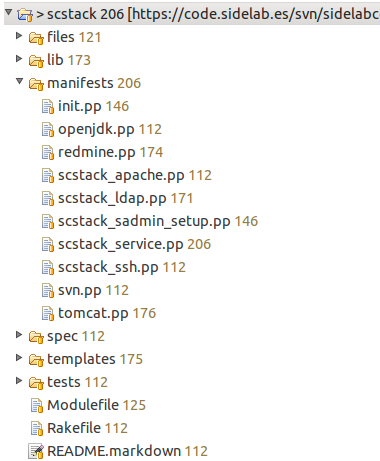
\includegraphics[width=0.5\textwidth]{sctack-puppet}
    \caption{Estructura de módulo Puppet de SCStack}
    \label{sctack-puppet}
\end{figure}

\par Pero no, no es suficiente ya que este manera el desarrollador ha de estar preocupado de invertir el tiempo en la gestión de las distintas máquinas virtuales, asignando espacio, potencia, configuración inicial, sobrecarga de la máquina de desarrollo y cumplir con una serie de tareas repetitivas que le alejan del camino marcado, el proyecto SidelabCode Stack.

\par En este punto aparece \emph{Vagrant}\footnote{Vagrant - \url{http://www.vagrantup.com/}}.

\begin{figure}[H]
    \centering
    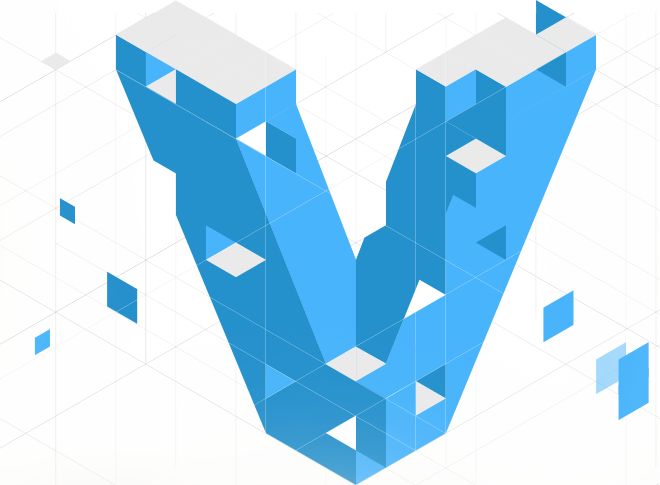
\includegraphics[width=0.3\textwidth]{vagrant}
    \caption{Vagrant Logo}
    \label{fir:vagrant}
\end{figure}

\begin{quote}
    \emph{Create a single file for your project to describe the type of machine you want, the software that needs to be installed, and the way you want to access the machine. Store this file with your project code.}
\end{quote}

\par Vagrant proporciona la gestión de los entornos de desarrollo sobre máquinas virtuales, ligeras, sencillas y replicables. Existe un repositorio de imágenes de virtuales\footnote{VagrantBox.es - \url{http://www.vagrantbox.es/}} preparadas para Vagrant que se han de instalar la máquina del desarrollador con un simple comando:

\lstset{style=bashbasico}
\begin{lstlisting}[frame=trbl]
config.vm.box = "precise64"
config.vm.network :hostonly, "192.168.33.10" # Si se desea se puede utilizar el modo bridge y asignar una ip por dhcp a la maquina dentro de la red en la que se encuentra el host
config.vm.provision :puppet, :module_path => "modules"
\end{lstlisting}

\par Se puede afirmar que Vagrant es la navaja suiza para las pruebas en este proyecto. A través de Vagrant se define el sistema operativo a instalar, la capacidad de la máquina y lo más importante: el \textbf{provisionador}, en nuestro caso Puppet y el módulo SidelabCode Stack.

\par A través de dos comandos se inicia el proceso completo de la instalación de SCStack en una nueva máquina virtual a partir de la configuración de una plantilla con las propiedades necesarias (Apéndice ~\ref{app:instalacion-sidelab}).

\lstset{style=bashbasico}
\begin{lstlisting}[frame=trbl]
$ vagrant box add base http://files.vagrantup.com/precise64.box
$ vagrant init
$ vagrant up
\end{lstlisting}

\par Permite la ejecución de pruebas para la instalación de SCStack de una manera eficiente y controlada aunque también es pesada debido a las características del proyecto.

\par De esta forma se completa el proceso de desarrollo con respecto a las herramientas y módulos utilizados para el desarrollo de la forja SidelabCode Stack ofreciendo las soluciones y herramientas necesarias para poder facilitar el uso del proceso desarrollo Iterativo e Incremental dentro de un marco seguro y fiable.

% subsection pruebas-instalacion (end)

% section pruebas-validacion (end)


%%%%%%%%%%%%%%%%%%%%%%%%%%%%%%%%%%%%%%

\chapter{Comunidades FLOSS}
\label{chap:comunidades}

\par El punto diferenciador en el proyecto haciendo hincapi\'e en la interacci\'on con las comunidades de software de cada una de las herramientas.

%%%%%%%%%%%%%%%%%%%%%%%%%%%%%%%%%%%%%%

%%%%%%%%%%%%%%%%%%%%%%%%%%%%%%%%%%%%%%%%%%%%%%%%%%%%%%%%%%%%%%%%%%%%%%%%%%%%%%%%%%%%%%%%%%%%%%%%%%%%%%%%%%%
%   \copyright 2013 Ricardo García Fernández - ricardogarfe [at] gmail [dot] com.
%
%    This work is licensed under a Creative Commons 3.0 Unported License.
%    To view a copy of this license visit:
% 
%    http://creativecommons.org/licenses/by/3.0/legalcode
%%%%%%%%%%%%%%%%%%%%%%%%%%%%%%%%%%%%%%%%%%%%%%%%%%%%%%%%%%%%%%%%%%%%%%%%%%%%%%%%%%%%%%%%%%%%%%%%%%%%%%%%%%

\chapter{Desarrollo de un proyecto}
\label{chap:desarrollo}

\par Cómo llevar a cabo el desarrollo de un proyecto con SCStack. Desde la creación de los usuarios y el proyecto hasta la definición del camino a seguir aplicando el desarrollo Iterativo e Incremental como los raíles del proceso. Generación de las distintas ramas del desarrollo adecuando la integración continua y marcando los objetivos dentro de una iteración a través de un grupo de tareas.

\par \textbf{Nota:}

\begin{quote}
    \emph{Si se quiere reproducir este proceso primero se ha de instalar la forja SCStack siguiendo los pasos descritos en el Apéndice ~\ref{app:instalacion-sidelab}.}
\end{quote}

\begin{comment}
Desarrollo en paralelo de un proyecto mediante github + travis-ci vs gerrit + jenkins.
\end{comment}

\section{Alta usuarios}
\label{sec:alta-usuarios}

\par El primer paso dar de alta a los usuarios a través de la Consola de Administración de la forja e incluirlos dentro de un grupo.

\par Se ha de aportar el nombre de usuario, correo electrónico y la contraseña. Ya se han creado los usuarios y éstos tienen acceso a todas las herramientas de SCStack.

\par \textbf{Nota:}

\begin{quote}
    \emph{Los nombres de usuario y proyecto han de cumplir con las reglas de usuarios propias de Redmine, como indica la validación de campos en el formulario.}
\end{quote}

% section alta-usuarios (end)

\section{Crear un proyecto}
\label{sec:crear-proyecto}

\par El siguiente paso es crear el proyecto.

\par Elegimos el nombre del proyecto, los usuarios y el grupo al que pertenecen.

\par Por último se elije si el proyecto ha de tener un repositorio, en este caso \textbf{si} y además ha de ser del tipo \textbf{Git}. Si el repositorio es público o privado no es vinculante para el proceso.

\par Ya disponemos de usuarios, grupos y proyecto al que pertenecen además de un repositorio Git asociado al nombre del nuevo proyecto que contiene dos ramas de desarrollo: \emph{master} y \emph{development}.

\subsection{Proyecto en redmine}
\label{sub:proyeto-redmine}

\par El administrador del nuevo proyecto accede a Redmine utilizando sus credenciales.

\par Se añade la lista de tareas a la Lista de Control.

\par Se define la historia de usuario a través de la interfaz del plugin \emph{Backlogs}.

\par Se crea el Sprint con las tareas seleccionadas a través del plugin \emph{Backlogs}.

\par Ya tenemos la lista de tareas que se van a completar en la primera iteración del proceso.

\par En el siguiente paso se prepara el entorno para los desarrolladores.

% subsection proyeto-redmine (end)

\subsection{Repositorio git}
\label{sub:repo-git}

\par El usuario, en este caso el desarrollador recibe sus credenciales para identificarse como tal en su equipo de trabajo.

\par El entorno de trabajo para el desarrollador en este caso consta de:

\begin{itemize}
	\item Equipo de trabajo con una distribución Ubuntu 12.04 LTS.
	\item Java JDK 1.6.
	\item Maven.
	\item Git-scm.
	\item Eclipse STS.
\end{itemize}

\par Configurar usuario Git del desarrollador de la forja:

\lstset{style=bashbasico}
\begin{lstlisting}[frame=trbl]
$ cat .gitconfig 
[user]
    name = ricardogarfe
    email = ricardogarfe@gmail.com
$ git config --global user.name "ricardogarfe"
$ git config --global user.email "ricardogarfe@gmail.com"
$ cd [path-to-gitrepo]
[path-to-gitrepo]$ git config user.name "ricardogarfe"
[path-to-gitrepo]$ git config user.email "ricardogarfe@gmail.com"
\end{lstlisting}

\par Comprobar las credenciales de Git en el ordenador del desarrollador:

\lstset{style=bashbasico}
\begin{lstlisting}[frame=trbl]
$ git config --list
    user.name=ricardogarfe
    user.email=ricardogarfe@gmail.com
\end{lstlisting}

% subsection repo-git (end)

\subsection{Configuración de Jenkins}
\label{sub:jenkins-configuracion}

\par Configuracón de Jenkins para realizar determinadas tareas de forma automática:

\begin{itemize}
	\item Tags
	\item Construir las versiones vivas
\end{itemize}

\par También proveerá tareas para ser ejecutadas manualmente:

\begin{itemize}
	\item Branches de releases
	\item Desplegar una versión específica con un clic
\end{itemize}

\par Las versiones vivas vivirán en su propia máquina virtual

\begin{figure}[H]
    \centering
    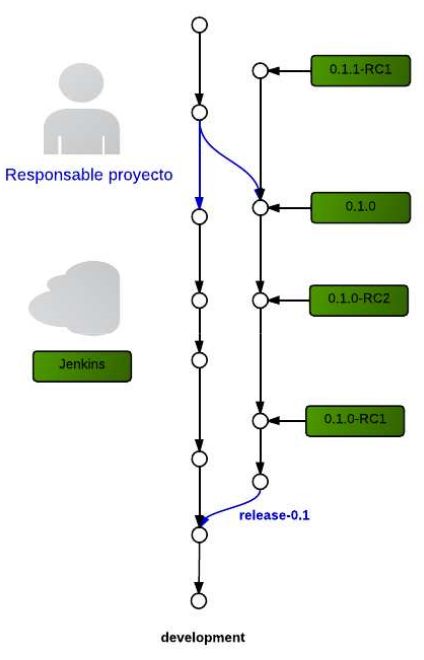
\includegraphics[width=0.6\textwidth]{jenkins-git}
    \caption{Jenkisn-Git relación en el proceso de integración}
    \label{fig:jenkins-git}
\end{figure}

\par Se mantendrán diferentes versiones vivas a la vez para cumplir unos objetivos con forme al desarrollo Iterativo e Incremental: \emph{'Release early, release often'}:

\begin{itemize}
	\item Asegurar la calidad
	\item Hacer el despliegue ágil
	\item Minimizar el riesgo
\end{itemize}

\par Para orientar la integración continua al proceso de desarrollo se ha de configurar \emph{Jenkins} para acceder a múltiples repositorios Git para esto se han de tener en cuenta los siguientes requerimientos:

\begin{itemize}
    \item \emph{Jenkins} construye diferentes proyectos en donde en proyecto puede tener su propio repositorio git.
    \item \emph{Jenkins} debe tener permisos de lectura o lectura/escritura a todos los repositorios de aquellos proyectos que vaya a construir.
    \item Por defecto \emph{Jenkins} usa la clave del usuario en \texttt{\ensuremath{\sim.ssh}} para autenticarse
    \item ¿Con qué usuario se ejecuta Jenkins? con el usuario \textbf{tomcat}.
\end{itemize}

\par El acceso de Jenkins a los distintos repositorios se configura a partir de un usuario por Jenkins repositorio, aislando los problemas descritos en la sección~\ref{sub:ci-jenkins} del capítulo \nameref{chap:procesos-desarrollo}.

\par Configurar \emph{Jenkins} para acceso a \emph{múltiples repositorios git} creando el usuario necesario en la Consola de Administración.

\begin{figure}[H]
    \centering
    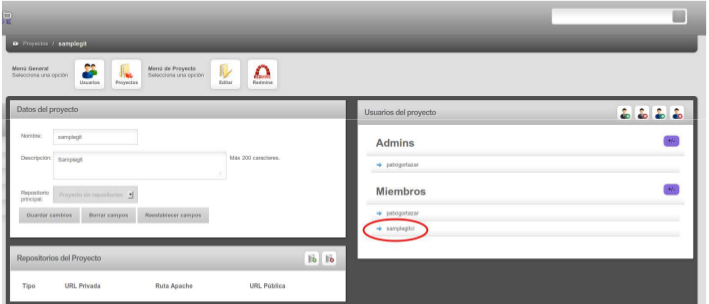
\includegraphics[width=\textwidth]{gestion-jenkins-usuarios-000}
    \caption{Crear usuarios para Jenkins a través de la consola de Administración}
    \label{fig:gestion-jenkins-usuarios-000}
\end{figure}

\par Generar un par de claves pública/privada con \texttt{ssh-keygen} para cada usuario en diferentes ficheros y acceder a Gerrit con cada usuario creado.

\begin{figure}[H]
    \centering
    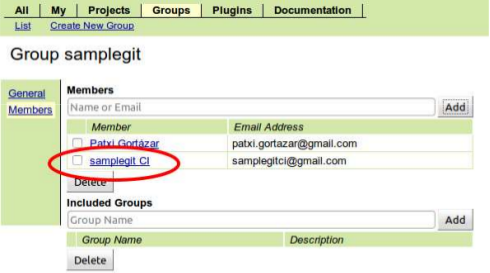
\includegraphics[width=\textwidth]{gestion-jenkins-usuarios-001}
    \caption{Configuración de usuarios Jenkisn en Gerrit}
    \label{fig:gestion-jenkins-usuarios-001}
\end{figure}

\par Añadir la clave pública para este usuario para copiar las claves al servidor de Jenkins en el directorio\texttt{'/opt/ssh-keys'}.

\lstset{style=bashbasico}
\begin{lstlisting}[frame=trbl]
$ git config --list
$ cd /opt/ssh-keys
$ ll
total 24
drwxr-xr-x  2 tomcat tomcat 4096 Jan  4 09:46 ./
drwxr-xr-x 14 root   root   4096 Jan  4 09:42 ../
- rw-------  1 tomcat tomcat 1679 Jan  4 09:46 filetransferci_rsa
- rw-r--r--  1 tomcat tomcat  398 Jan  4 09:46 filetransferci_rsa.pub
- rw-------  1 tomcat tomcat 1679 Jan  4 09:44 samplegitci_rsa
- rw-r--r--  1 tomcat tomcat  396 Jan  4 09:44 samplegitci_rsa.pub
</code>
\end{lstlisting}

\par Configurar SSH con la clave correcta creando el fichero \texttt{'/home/tomcat/.ssh/config'}.

\lstset{style=bashbasico}
\begin{lstlisting}[frame=trbl]
$ git config --list
$ cd /home/tomcat/.ssh
$ cat config
Host samplegit.ricardogarfe.sidelab.es
    HostName ricardogarfe.sidelab.es
    User samplegitci
    IdentityFile /opt/ssh-keys/samplegitci_rsa
Host filetransfer.ricardogarfe.sidelab.es
    HostName ricardogarfe.sidelab.es
    User filetransferci
    IdentityFile /opt/ssh-keys/filetransferci_rsa
\end{lstlisting}

\subsection{Configuración de builds}
\label{sub:jenkins-build-jobs}

\par Los builds de \emph{Jenkins} funcionan a través de la configuración de \textbf{jobs}. Por lo que vamos a definir los jobs necesarios para el proceso de integración continua. Se dividen en tres grupos:

\begin{itemize}
    \item Jobs de \textbf{integración} (read only).
        \begin{itemize}
            \item Descargan el código (checkout).
            \item Construyen.
            \item Pasan tests.
            \item Despliegan la versión construida en ``local''.
        \end{itemize}
    \item Jobs de \textbf{release} (read/write).
        \begin{itemize}
            \item Realizan los pasos anteriores y además.
            \item Tag si los tests pasaron.
            \item Push del tag al repositorio remoto.
        \end{itemize}
    \item Jobs de \textbf{despliegue} (read only).
        \begin{itemize}
            \item Descargan el binario del repositorio de binarios
            \item Desplegar
        \end{itemize}
\end{itemize}

\subsubsection{Job de integración}
\label{subs:jenkins-job-integracion}

\par Configurar el Job de integración mediante Maven para asegurar la fiabilidad dentro de cada iteración en el desarrollo:

\begin{itemize}
	\item Crear un \textbf{job} \emph{Maven}.
	\item Configurar el repositorio git:
        \begin{itemize}
	        \item \emph{ssh://filetransferci@filetransferci.code.tscompany.es/filetransfer}
	        \item Ssh leerá el fichero config y utilizará el fichero de claves correspondiente el host \texttt{filetransferci.code.tscompany.es}.
        \end{itemize}
	\item Añadir las ramas a construir (añadir nuevas ramas con el botón ``Add'')
        \begin{itemize}
	        \item development
	        \item release-0.1.1
        \end{itemize}
	\item Añadir el \texttt{user.email} y \texttt{user.name} que usará \emph{Jenkins}.
        \begin{figure}[H]
            \centering
            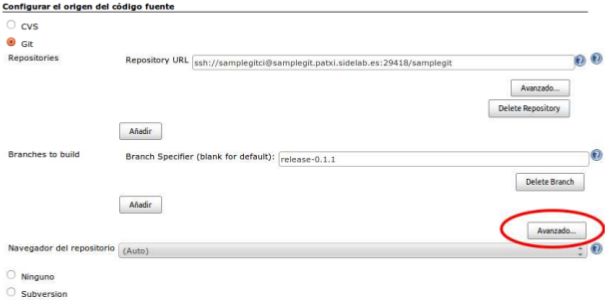
\includegraphics[width=0.7\textwidth]{jenkins-job-integracion}
            \caption{Crear Job integración en Jenkins}
            \label{fg:jenkins-job-integracion}
        \end{figure}
	\item Los resultados del build se pueden comprobar en: 
        \begin{itemize}
	        \item \texttt{/opt/jenkins/jobs/filetransfer/workspace}
	        \item Si es un proyecto \emph{Maven}, dentro del proyecto en la carpeta target estará el artefacto generado.
	        \item También se puede acceder vía web y descargar el workspace como un zip.
	        \item Los \textbf{tests} están en la carpeta \texttt{surfire-reports} del proyecto \emph{Maven}.
	        \item También pueden consultarse vía web accediendo al build y seleccionando \emph{'Resultado de los tests'}.
        \begin{figure}[H]
            \centering
            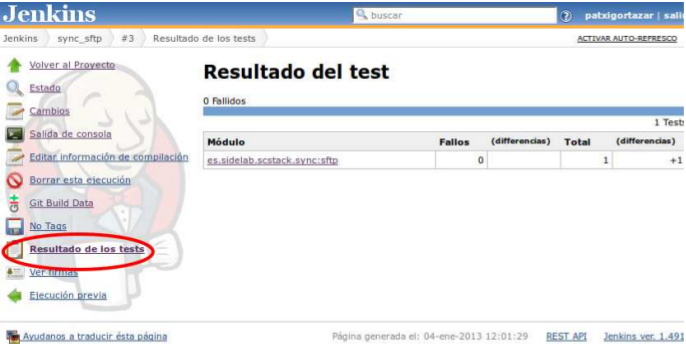
\includegraphics[width=\textwidth]{jenkins-job-resultados}
            \caption{Resultados de los test a través de la interfaz de Jenkins}
            \label{fig:jenkins-job-resultados}
        \end{figure}
        \end{itemize}
\end{itemize}

\subsection{Maven}
\label{sub:jenkins-maven}

\par \emph{Jenkins} permite construir proyectos \emph{Maven}.

\par En determinadas ocasiones los proyectos requieren configuraciones específicas. La información sensible suele ir en el fichero \texttt{settings.xml} en el \texttt{home} del usuario en su máquina de desarrollo.

\begin{itemize}
    \item Info de \textbf{autenticación para Archiva}.
    \item \textbf{Profiles}
\end{itemize}

\par En Jenkins esto se puede gestionar con el plugin \emph{``Config File Provider Plugin''}.

\begin{figure}[H]
    \centering
    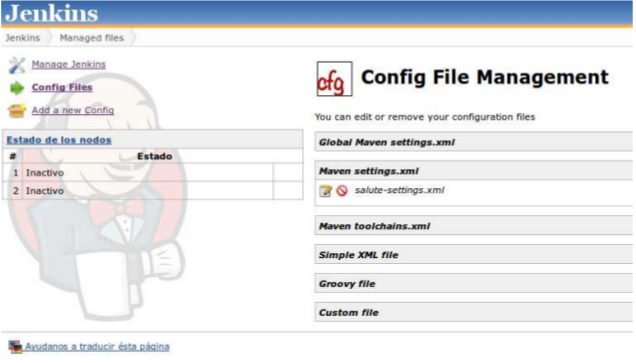
\includegraphics[width=\textwidth]{jenkins-config-file-management}
    \caption{Configuración de Maven a través de Jenkins}
    \label{fig:jenkins-config-file-management}
\end{figure}

\par Podemos añadir cualquiera de los ficheros creados con \emph{Config File Management} en un \textbf{job}.

\begin{figure}[H]
    \centering
    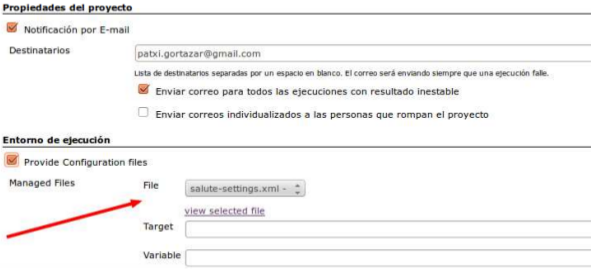
\includegraphics[width=\textwidth]{jenkins-config-file-management-settings}
    \caption{Seleccionar archivo de configuración de Maven}
    \label{fig:jenkins-config-file-management-settings}
\end{figure}

\par Para los despliegues, si el certificado es \emph{autofirmado} es \textbf{necesario} generar un \textbf{truststore} a partir del certificado generado por el servidor\footnote{\url{http://www.liferay.com/web/neil.griffin/blog/-/blogs/fixing-suncertpathbuilderexception-caused-by-maven-downloading-from-self-signed-repository}}.

\par Este \textbf{truststore} debe incluirse en todos los \texttt{jdk} que utilice \emph{Jenkins} en la ruta indicada en el enlace anterior.

% subsection jobs-jenkins (end)

% section crear-proyecto (end)

\section{Proceso de desarrollo basado en ramas}
\label{sec:desarrollo-en-ramas}

\par Después completar la configuración del entorno de desarrollo y la forja SCStack, es el turno aplicar el proceso Iterativo e Incremental al código fuente a través del repositorio Git.

\par El flujo de trabajo a través de las ramas se representa en este \emph{Diagrama de Desarrollo} en el que intervienen e interactúan las distintas ramas durante el proceso de Integración dentro de cada Iteración:

\begin{figure}[H]
    \centering
    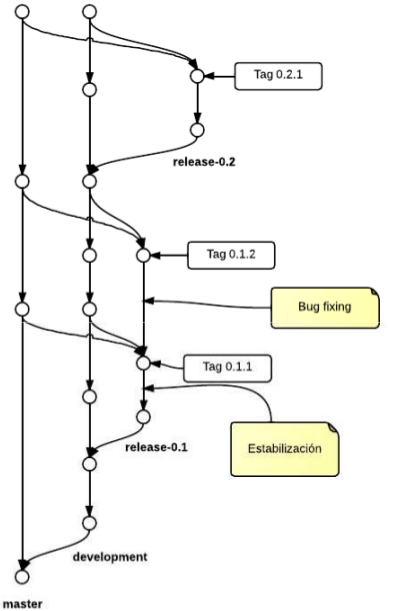
\includegraphics[width=0.6\textwidth]{flujo-desarrollo-git-000}
    \caption{Flujo de desarrollo Git basado en ramas}
    \label{fig:flujo-desarrollo-git-000}
\end{figure}

\par Se ha definido que el proceso de desarrollo basado en ramas parte de 2 ramas de forma continua:

\begin{itemize}
    \item \textbf{master:} Desarrollo limpio. Sólo versiones estables.
    \item \textbf{develop:} El desarrollo inicial de la versión actual tiene lugar aquí.
\end{itemize}

\par En cada iteración se han de gestionar las ramas para estabilización de las iteraciones, en este caso se utiliza el nombre de \emph{release} acompañado de la etiqueta numérica asociada:

\begin{itemize}
    \item \textbf{release-0.1}, \textbf{release-0.2}; una rama de estabilización cada vez   
\end{itemize}

\par El siguiente proceso se conoce como \emph{proceso de estabilización} y se gestiona a través de las \emph{ramas de estabilización}. Es un paso intermedio de integración del as ramas de estabilización (release-0.1, 0.2) y las ramas continuas (master y development):

\begin{itemize}
    \item Estabilización del código (\emph{RC release candidates})
    \item Arreglar bugs (hotfixes)
    \item Cuando la versión se considera estable se procede al siguiente paso:
        \begin{itemize}
            \item Tag
            \item Mezclar (merge) con development
            \item Mezclar (merge) con master
        \end{itemize}
    \item Si surgen nuevos bugs se vuelve a repetir el \textbf{proceso de estabilización}:
        \begin{itemize}
            \item Se arreglan en la misma rama (release-0.1)
            \item Nuevo tag y mezcla
        \end{itemize}
\end{itemize}

\subsection{Releasing}

\par Para crear una \emph{Release} se define un proceso de gestión a través las ramas:

\begin{itemize}
    \item Checkout del tag
    \item Build (Jenkins)
    \item Deploy (Jenkins)
\end{itemize}

% section desarrollo-en-ramas (end)

%%%%%%%%%%%%%%%%%%%%%%%%%%%%%%%%%%%%%%

%%%%%%%%%%%%%%%%%%%%%%%%%%%%%%%%%%%%%%

\chapter{Ep\'ilogo}
\label{chap:epilogo}

\section{Conclusiones}
\label{sec:conclusiones}

\par El uso de estas herramientas y su incremento de la calidad en el desarrollo, por encima de todo siendo FLOSS debido a eso la versatilidad que otorga en el momento de unificarlas en una herramienta nueva; SidelabCode Stack.


\section{Lecciones aprendidas}
\label{sec:lecciones}

\par Colaboraci\'on entre distintos proyectos y comunidades, interoperabilidad entre herramientas, Forjas de desarrollo y los elementos m\'as comunes de las mismas.

\section{Trabajo Futuro}
\label{sec:trabajofuturo}

\par Impulso de la comunidad a trav\'es de los canales habituales.

\par Integraci\'on y gesti\'on de nuevas herramientas comunes para los desarrolladores.

\par Centralizaci\'on de la instalaci\'on.

% section epilogo (end)

%%%%%%%%%%%%%%%%%%%%%%%%%%%%%%%%%%%%%%

\appendix
\clearpage % o \cleardoublepage
\addappheadtotoc
\appendixpage

% Puppet proyecto de ejemplo.
%%%%%%%%%%%%%%%%%%%%%%%%%%%%%%%%%%%%%%%%%%%%%%%%%%%%%%%%%%%%%%%%%%%%%%%%%%%%%%%%%%%%%%%%%%%%%%%%%%%%%%%%%%%
%   \copyright 2013 Ricardo García Fernández - ricardogarfe [at] gmail [dot] com.
%
%    This work is licensed under a Creative Commons 3.0 Unported License.
%    To view a copy of this license visit:
% 
%    http://creativecommons.org/licenses/by/3.0/legalcode
%%%%%%%%%%%%%%%%%%%%%%%%%%%%%%%%%%%%%%%%%%%%%%%%%%%%%%%%%%%%%%%%%%%%%%%%%%%%%%%%%%%%%%%%%%%%%%%%%%%%%%%%%%

\chapter{Puppet}
\label{app:apendice-puppet}

\par Instalación de Puppet siguiendo la documentación ofrecida en su página web\footnote{Puppet Documentation - \url{http://docs.puppetlabs.com/guides/installation.html\#debian-and-ubuntu}}.

\par El proceso automatiza la instalación y configuración manual de un componente, un servidor web.

\begin{itemize}
	\item Primero se ha de crear la instalación manual del servidor en un entorno definido (Sistema operativo Ubuntu). Configurar los permisos, definir archivos de configuración, directorios a servir, públicos/privados.
	\item Recapitular todos los pasos seguidos en la instalación y la información sobre la configuración para reescribirla a un módulo Puppet.
	\item Crear el esqueleto del módulo Puppet.
	\item Definir las órdenes a ejecutar organizando el módulo en distintas clases y apartados cada una responsable de una funcionalidad.
	\begin{itemize}
	    \item Descargar servidor web.
	    \item Instalar servidor web.
	    \item Configurar servidor web a través de una plantilla Ruby basada en los ficheros de configuración base del servidor web. Directorios, usuarios, urls, dominios, web de bienvenida, etc.
	    \item Poner en marcha el servidor.
    \end{itemize}
\end{itemize}

\par Puppet da la opción de publicar los módulos desarrollados en un repositorio central de módulos para que estén accesibles para los usuarios de Puppet con un sistema de búsqueda para ayudar a los usuarios.

\par Con este módulo Puppet podemos replicar la instalación en cualquier entorno con tan solo ejecutar el módulo a través de Puppet para la ejecución. Descargar el módulo y ejecutar el commando Puppet.

\par Código Puppet de ejemplo para la instalación del servidor web Apache a través del módulo Puppet publicado en PuppetForge\footnote{Pupept Apache Module - \url{https://forge.puppetlabs.com/puppetlabs/apache}}:

\par Instalar Apache importando la clase del módulo:

\lstset{style=rubybasico}
\begin{lstlisting}[frame=trbl]
class {'apache':  }
\end{lstlisting}

\par Módulo PHP de Apahce:

\lstset{style=rubybasico}
\begin{lstlisting}[frame=trbl]
class {'apache::mod::php': }
\end{lstlisting}

\par Configurar Host Virtual mediante los distintos parámetros de configuración, partiendo del mínimo un ejemplo sería este:

\lstset{style=rubybasico}
\begin{lstlisting}[frame=trbl]
apache::vhost { 'www.example.com':
    priority        => '10',
    vhost_name      => '192.0.2.1',
    port            => '80',
}
\end{lstlisting}

\par Se pueden definir más parámetros de configuración:

\lstset{style=rubybasico}
\begin{lstlisting}[frame=trbl]
apache::vhost { 'www.example.com':
    priority        => '10',
    vhost_name      => '192.0.2.1',
    port            => '80',
    docroot         => '/home/www.example.com/docroot/',
    logroot         => '/srv/www.example.com/logroot/',
    serveradmin     => 'webmaster@example.com',
    serveraliases   => ['example.com',],
}
\end{lstlisting}

% subsection puppet-caso-de-uso (end)

% section puppet (end)

% Instalación SidelabCode Stack
%%%%%%%%%%%%%%%%%%%%%%%%%%%%%%%%%%%%%%%%%%%%%%%%%%%%%%%%%%%%%%%%%%%%%%%%%%%%%%%%%%%%%%%%%%%%%%%%%%%%%%%%%%%
%   \copyright 2013 Ricardo García Fernández - ricardogarfe [at] gmail [dot] com.
%
%    This work is licensed under a Creative Commons 3.0 Unported License.
%    To view a copy of this license visit:
% 
%    http://creativecommons.org/licenses/by/3.0/legalcode
%%%%%%%%%%%%%%%%%%%%%%%%%%%%%%%%%%%%%%%%%%%%%%%%%%%%%%%%%%%%%%%%%%%%%%%%%%%%%%%%%%%%%%%%%%%%%%%%%%%%%%%%%%

\chapter{Instalación SidelabCode Stack}
\label{app:instalacion-sidelab}

\par En la versión 0.4 de SidelabCode Stack se utiliza Puppet en el proceso de instalación. Ahora es extremadamente sencillo instalar SidelabCode Stack usando Puppet o Vagrant con el nuevo instalador.

\par Puppet nos permite automatizar la instalación en un servidor \emph{Ubuntu} mediante una sencilla configuración.

\par El uso de \emph{Vagrant} permite probar SidelabCode Stack en una máquina virtual en 5 minutos.

\section{Requisitos}
\label{sec:requisitos}

\par Para la instalación de SidelabCode Stack es necesario obtener los siguientes recursos.

\par Dependiendo de la instalación que se utilice \textbar{Vagrant} o \textbar{Puppet} se han de seguir instrucciones diferentes.

\subsection{Descarga SidelabCode Stack}
\label{sub:descarga}

\par Descargar el instalador de SidelabCode Stack (módulo scstack) y sus dependencias de la url:

\begin{itemize}
	\item \url{http://code.sidelab.es/public/sidelabcodestack/artifacts/0.3/puppet-installer-0.3-bin.tar.gz}
\end{itemize}

\lstset{style=rubybasico}
\begin{lstlisting}[frame=trbl]
    cd $HOME
    mkdir tmp
    cd $HOME/tmp
    wget http://code.sidelab.es/public/sidelabcodestack/artifacts/0.3/puppet-installer-0.3-bin.tar.gz
\end{lstlisting}

\par Descomprimir y copiar a la carpeta modules:

\lstset{style=rubybasico}
\begin{lstlisting}[frame=trbl]
    cd $HOME/tmp
    tar xvzf puppet-installer-0.3-bin.tar.gz
\end{lstlisting}

\subsection{Configuración de módulos puppet}
\label{sub:conf-modulos-puppet}

\par Creamos un fichero \texttt{default.pp} en la carpeta \texttt{tmp} con el siguiente contenido:

\lstset{style=rubybasico}
\begin{lstlisting}[frame=trbl]
    exec { "apt-update":
        command => "/usr/bin/apt-get update",
    }
    class { "scstack":
        # Superadmin password. Will be used to access the SidelabCode Stack Console re@lity45
        sadminpass => "re@lity45",
        # Or whatever IP specified in Vagrantfile
        ip => "192.168.33.10", 
        domain => "sidelabcode03.scstack.org",
        baseDN => "dc=sidelabcode03,dc=scstack,dc=org",
        # Your company/organization name
        compname => "SidelabCode Stack version 0.3",
        # A name to be displayed within Redmine
        codename => "SCStack ALM Tools",
    }
\end{lstlisting}

\subsection{Apt Cacher}
\label{sub:apt-cacher}

\par Dependiendo de la conexión de red, el proceso de instalación puede tardar más o menos. En general es buena idea configurar un proxy para los paquetes debian. Esta opción es recomendable en el proceso de instalación a través de Vagrant. Para ello, simplemente hay que instalar \textbf{apt-cacher} en el host:

\lstset{style=rubybasico}
\begin{lstlisting}[frame=trbl]
    sudo apt-get install apt-cacher
\end{lstlisting}

\par Modificar las siguientes líneas del fichero \emph{/etc/apt-cacher/apt-cacher.conf}:

\lstset{style=rubybasico}
\begin{lstlisting}[frame=trbl]
    daemon_addr = 192.168.33.1 # No podemos usar localhost si queremos que los clientes se puedan conectar
    allowed_hosts = * # Permitir a todos los clientes conectarse a este proxy.
    generate_reports = 1 # Generar un informe cada 24h
\end{lstlisting}

\par Reiniciar el servicio:

\lstset{style=rubybasico}
\begin{lstlisting}[frame=trbl]
    sudo /etc/init.d/apt-cacher restart
\end{lstlisting}

\par Modificar el fichero \texttt{/etc/hosts} con la ip del host y el dominio asociado que se define en el fichero de configuración \texttt{default.pp} y la ip y el dominio del cliente para la comunicación con \texttt{apt-cacher} definido en el parámetro \texttt{daemon\_addr} del fichero \texttt{/etc/apt-cacher/apt-cacher.conf}:

\lstset{style=rubybasico}
\begin{lstlisting}[frame=trbl]
    192.168.33.10   sidelabcode03.scstack.org
    192.168.33.1    host.scstack.es
\end{lstlisting}

\par Añadir el siguiente trozo de código en la primera línea del fichero \texttt{default.pp} para que utilice el apt-cacher creado:

\lstset{style=rubybasico}
\begin{lstlisting}[frame=trbl]
    file { "/etc/apt/apt.conf.d/01proxy":
        content => 'Acquire::http::Proxy "http://192.168.33.1:3142/apt-cacher";',
    }
\end{lstlisting}

\section{Vagrant}
\label{sec:vagrant}

\par La instalación a través de Vagrant permite probar SidelabCode Stack en una máquina virtual en 5 minutos.

\subsection{Descripción del entorno de instalación}
\label{sub:entorno-instalacion}

\par Básicamente lo que vamos a hacer es indicar a Vagrant que monte una red privada entre la máquina host y la máquina virtual donde instalaremos SidelabCode Stack. Esto nos permite tener acceso a la forja desde el host. Normalmente, Vagrant asigna, dentro de esa red privada, la IP 192.168.33.1 al host y la IP 192.168.33.10 a la máquina virtual. Estos valores se pueden cambiar como veremos posteriormente.

\subsection{Prerequisitos}
\label{sub:prerequisitos}

\begin{itemize}
    \item Instalar Vagrant y Virtualbox (descargar las últimas versiones de las respectivas páginas web)
    \item Añadir Vagrant al path
\end{itemize}

\lstset{style=rubybasico}
\begin{lstlisting}[frame=trbl]
    $ gedit $HOME/.bashrc
    $ PATH=$PATH:/opt/vagrant/bin
\end{lstlisting}

\subsection{Preparación de la VM}
\label{preparar-vm}

\par Utilizaremos Vagrant para provisionar una VM con Java donde poder instalar SidelabCode Stack. Preparamos la carpeta para el proyecto Vagrant.

\lstset{style=rubybasico}
\begin{lstlisting}[frame=trbl]
    mkdir vagrant
    mkdir vagrant/manifests
    mkdir vagrant/modules
\end{lstlisting}

\par Descargar una imagen vagrant (precise64 es la que elegimos en esta documentación, por ser LTS).

\lstset{style=rubybasico}
\begin{lstlisting}[frame=trbl]
    vagrant box add precise64 http://files.vagrantup.com/precise64.box
\end{lstlisting}

\par Si quiere utilizar una versión distinta de una distribución, puede seleccionarla en la lista de \textbf{boxes} que proporciona \href{http://www.vagrantbox.es/}{vagrant para virtualbox}.

\par Crear un proyecto Vagrant:

\lstset{style=rubybasico}
\begin{lstlisting}[frame=trbl]
    vagrant init
\end{lstlisting}

\par Modificar el Vagrantfile que describe el proyecto (VM, provisioner, etc) para que arranque la vm ``precise64'' y utilice Puppet:

\lstset{style=rubybasico}
\begin{lstlisting}[frame=trbl]
config.vm.box = "precise64"
config.vm.network :hostonly, "192.168.33.10" # Si se desea se puede utilizar el modo bridge y asignar una ip por dhcp dentro de la red en la que se encuentra el host
config.vm.provision :puppet, :module_path => "modules"

\end{lstlisting}

\par Copiar el instalador de la forja en la carpeta modules del proyecto Vagrant:

\lstset{style=rubybasico}
\begin{lstlisting}[frame=trbl]
    cp -R puppet-installer-0.3/* $HOME/vagrant/modules
\end{lstlisting}

\par Copiar el fichero \texttt{default.pp} en la carpeta \texttt{manifests} del proyecto Vagrant:

\lstset{style=rubybasico}
\begin{lstlisting}[frame=trbl]
    cp /tmp/default.pp $HOME/vagrant/manifests
\end{lstlisting}

\par Arrancar la vm.

\lstset{style=rubybasico}
\begin{lstlisting}[frame=trbl]
    cd $HOME/vagrant
    vagrant up
\end{lstlisting}

\section{Puppet}
\label{puppet}

\textbf{TBC}: Descripción

\subsection{Pre requisitos}
\label{sub:puppet-pre-requisitos}

\par Puppet se ha de instalar mediante el gestor de paquetes de la distribución, en este caso \texttt{apt} para Ubuntu:

\lstset{style=rubybasico}
\begin{lstlisting}[frame=trbl]
    $ [sudo] apt-get install puppet
\end{lstlisting}

\par La instalación en otras distribuciones se puede consultar en el \href{http://docs.puppetlabs.com/guides/installation.html}{manual de puppet}.

\subsection{Configuración}
\label{sub:configuracion-puppet}

\par Copiar los módulos puppet al directorio de módulos definido:

\lstset{style=rubybasico}
\begin{lstlisting}[frame=trbl]
    $ mkdir -p $HOME/puppet/modules
    $ cp -R puppet-installer-0.3/* $HOME/puppet/modules
\end{lstlisting}

\par Ejecutar puppet para el proceso de instalación mediante sudo:

\lstset{style=rubybasico}
\begin{lstlisting}[frame=trbl]
    $ sudo puppet apply --modulepath=$HOME/puppet/modules default.pp
\end{lstlisting}

\section{Post instalación}
\label{sec:post-instalacion}

\par El proceso de instalación comenzará automáticamente. Una vez finalizado, en la dirección
\href{http://test.scstack.org/redmine}{http://test.scstack.org/redmine} se mostrará Redmine. La consola es accesible a través de la dirección \href{https://test.scstack.org:5555}{https://test.scstack.org:5555}. Es posible administrar scstack accediendo con el usuario \emph{sadmin} y la contraseña especificada en el parámetro \emph{sadminpass}.

\par \textbf{Nota:} La consola de administración se ha comprobado el funcionamiento para los siguientes navegadores:

\begin{itemize}
	\item \href{http://www.mozilla.org/es-ES/firefox/new/}{Firefox}.
	\item \href{https://www.google.com/intl/es/chrome/browser/?hl=es}{Chrome/Chromium}

\end{itemize}

\subsection{Primeros pasos}
\label{sub:primeros-pasos}

\par Después de la instalación automatizada del entorno se ha de acceder a las herramientas \textbf{Redmine} y \textbf{Archiva} para completar el proceso.

\par Antes de nada se ha de reiniciar la máquina para comprobar que se ejecutan todos los procesos en el inicio.

\subsubsection{Redmine}
\label{subs:conf-redmine}

\par odificar la fecha de creación de la api key de admin desde mysql:

\lstset{style=rubybasico}
\begin{lstlisting}[frame=trbl]
mysql -u root -p
> use redminedb;
> update tokens set created_on='2013-01-16 22:16:00' where id='1';
\end{lstlisting}

\par Modificar los permisos de las carpetas en /opt/redmine/tmp para que sean del usuario de apache:

\begin{itemize}
\item
  \texttt{cd /opt/redmine/tmp \&\& chown -R www-data:www-data *}
\end{itemize}
Acceder a la URL de Redmine, con el usuario \texttt{admin} y el password
\texttt{admin}:

\begin{itemize}
\item \href{https://test.scstack.org/redmine}{https://test.scstack.org/redmine}
\end{itemize}

\par Cambiar la contraseña para que no utilice la genérica a través de la ruta:

\begin{itemize}
\item Administración \textgreater{} Users \textgreater{} admin \textgreater{} Authentication \textgreater{} actualizar.
\end{itemize}

\par Cambiar la API key para securizar el acceso a la API rest (scstack instala una por defecto, pero no es segura):

\begin{itemize}
    \item Acceder como admin \textgreater{} My account \textgreater{} API  access key \textgreater{} Reset \textgreater{} Show -\textgreater{} Copiar la key
    \item Pegar la key en el fichero /opt/scstack-service/scstack.conf
    \item Reiniciar el servicio scstack: \texttt{sudo service scstack-service restart}
\end{itemize}

\subsubsection{Gerrit}
\label{subs:conf-gerrit}

\par El primer usuario que accede a Gerrit obtiene privilegios de administrador. Al instalar la forja, se recomienda crear un usuario ``gerritadmin'' y password ``t0rc0zu310'' y acceder con este usuario a Gerrit. Este usuario se convertirá en administrador automáticamente al hacer login. A partir de este momento, este será el usuario con el que crear los grupos y proyectos (repositorios) en Gerrit.

\par Obtener la clave pública del servidor para asignarla al usuario \textbf{gerritadmin}:

\begin{enumerate}
\item \emph{Settings \textgreater{} SSH Public Keys}\textgreater{} Add.
\item Copiar la clave del fichero \texttt{/opt/ssh-keys/gerritadmin\_rsa.pub}.
\end{enumerate}

\par Configurar permisos para creación de proyectos:

\begin{enumerate}
    \item Acceder a \emph{Projects \textgreater{} List}\textgreater{} All-Projects.
    \item Seleccionar \emph{Access}:
    \item \emph{Editar}:
    \begin{itemize}
	    \item \texttt{Bloque} \textbf{refs/} Add Permission \textgreater{} añadir \emph{Push} el grupo \emph{Administrators}.
	    \item \texttt{Bloque} \textbf{refs/meta/config} Add Group \textgreater{} añadir a \emph{Read} el grupo \emph{Administrators}.
	    \item Save Changes.
    \end{itemize}
\end{enumerate}


\subsubsection{Archiva}
\label{subs:conf-archiva}

\par Acceder a la URL de Archiva:

\begin{itemize}
    \item \url{https://test.scstack.org/archiva}
\end{itemize}

\par La primera vez que se configura archiva pide los datos del administrador. Apuntarlos convenientemente para posteriores necesidades de administración. Se recomienda utilizar la contraseña del administrador de la forja definida en el fichero de configuración \texttt{default.pp}.

\paragraph{Repositorios}

\par Por defecto, Archiva trae configurado un \textbf{repositorio internal} que hace de proxy de \emph{Maven Central} y \emph{java.net}. Si hace falta añadir repositorios remotos adicionales, en Repositories, al final de la página se pueden añadir repositorios remotos.

\par Archiva trae configurado un \textbf{repositorio de snapshots}. Se recomienda crear uno de \textbf{releases}.

\par Para ello accedemos a la administración de Archiva \texttt{Administration -\textgreater{} Repositories} y añadimos uno nuevo con los siguientes parámetros:

\lstset{style=rubybasico}
\begin{lstlisting}[frame=trbl]
Identifier*: *releases*
Name*:       *Archiva Managed Releases Repository*
Directory*:  */opt/tomcat/data/repositories/releases*
...
Repository Purge By Days Older Than: *30*
\end{lstlisting}

\par Se crea el repositorio. Si Tomcat nos muestra un error por pantalla al acceder a la URL \texttt{https://test.scstack.org/archiva/admin/addRepository!commit.action} relacionado con \textbf{NullPointerException} no nos debemos preocupar ya que el repositorio está creado correctamente siendo accesible y funcional. Se puede comprobar volviendo a visualizar la lista de repositorios de \emph{Archiva}.

\paragraph{Usuarios}

\par Archiva no lee los usuarios de \emph{OpenLDAP}, por tanto es necesario añadirlos a mano. En principio, debería ser suficiente con un \textbf{usuario de deploy} para \emph{toda la organización}, o como mucho, un usuario por proyecto o grupo de proyectos.

\par El usuario debe ser \textbf{Observer} de los tres repositorios y \emph{\textbf{manager} de} snapshots y releases.

\section{FAQ}
\label{sec:faq}

\par Posibles problemas que se pueden encontrar tras la instalación:

\begin{itemize}
    \item Error al crear un repositorio Git: Reininciar el servicio scstack-service:
    \lstset{style=rubybasico}
    \begin{lstlisting}[frame=trbl]
        $sudo service scstack-service stop
        $sudo service scstack-service start
    \end{lstlisting}

    \item Error al acceder a \textbf{Archiva} o \textbf{Jenkins} \texttt{404 No encontrado}.
    \begin{itemize}
        \item Configurar el dominio de nombres en el ordenador para que acceda a través de la ip correspondiente.

        \lstset{style=rubybasico}
        \begin{lstlisting}[frame=trbl]
            $ sudo vi /etc/hosts
        \end{lstlisting}

        \item Añadir la línea de conversión entre IP y nombre (elegido en la configuración del fichero default.pp).

        \lstset{style=rubybasico}
        \begin{lstlisting}[frame=trbl]
            138.100.156.246 sidelabcode03.scstack.org
        \end{lstlisting}
     \end{itemize}
\end{itemize}


%%%%%%%%%%%%%%%%
% BIBLIOGRAFIA %
%%%%%%%%%%%%%%%%

\begin{comment}
    Referenciar bibliografía: reference 1 ~\cite{New-commercial-OSS-standford-2010}.
\end{comment}

\begin{thebibliography}{25}
\bibliographystyle{alpha}

\bibitem{larman2003iterative} Larman, Craig and Basili, Victor R. \textit{Iterative and incremental developments. a brief history}. IEEE, 2003.

\bibitem{featurebranch} Fowler, Martin. \textit{Feature Branch}. http://martinfowler.com/bliki/FeatureBranch.html, September 2009.

% Forjas

\bibitem{cenatic-forjas} Jose Angel Diaz Diaz Manuel Velardo Pacheco. \textit{INFORME TÉCNICO Forjas: entornos de desarrollo colaborativo. Su integración en el ámbito empresarial.}. CENATIC (Centro Nacional de Referencia de Aplicación de las TIC basadas en fuentes abiertas), 2009.

\bibitem{open-collaboration-forges} Dirk Riehle, John Ellenberger, Tamir Menahem, Boris Mikhailovski, Yuri Natchetoi, Barak Naveh, Thomas Odenwald. \textit{Open Collaboration within Corporations Using Software Forges}. IEEE Software, March/April 2009.

\bibitem{yodemayorforja} Micael gallego. \textit{Mamá, yo de mayor quiero una forja (de desarrollo software)}. \url{http://sidelab.wordpress.com/2011/07/05/mama-yo-de-mayor-quiero-una-forja-de-desarrollo-software/}, 2011.

\bibitem{google-code-open} Jonathan Rosenberg. \textit{The meaning of open}. Google Official Blog \url{http://googleblog.blogspot.com.es/2009/12/meaning-of-open.html}, December 2009.

\bibitem{comparativa-forjas-wiki} Wikipedia. \textit{Comparison of open-source software hosting facilities}. \url{http://en.wikipedia.org/wiki/Comparison_of_open_source_software_hosting_facilities}, 2013.

\bibitem{bitergia-fusionforge-analysis} Jesus M. Gonzalez-Barahona, \textit{The history of FusionForge and GForge}. \url{http://blog.bitergia.com/2012/11/16/the-history-of-fusionforge-and-gforge/}, Bitergia's blog, November 16 2012

\bibitem{clean-code} Robert C. Martin, \textit{Clean Code}, Chapter 9 Unit Test, Prentice Hall, 2008.

\end{thebibliography}

\end{document}
